\documentclass[conference]{IEEEtran}
\IEEEoverridecommandlockouts
% The preceding line is only needed to identify funding in the first footnote. If that is unneeded, please comment it out.
\usepackage{cite}
\usepackage{amsmath,amssymb,amsfonts}
\usepackage{algorithmic}
\usepackage{graphicx}
\usepackage{float}
\usepackage{textcomp}
\usepackage{xcolor}
\def\BibTeX{{\rm B\kern-.05em{\sc i\kern-.025em b}\kern-.08em
    T\kern-.1667em\lower.7ex\hbox{E}\kern-.125emX}}
\begin{document}

\title{Quadrature Down Converter\\
}

\author{\IEEEauthorblockN{Advaith Sudarshan}
\IEEEauthorblockA{\textit{2024102021} \\
\textit{IIIT Hyderabad}\\
\textit{ECD}\\
\text{advaith.sudarshan\\@research.iiit.ac.in}}
\and
\IEEEauthorblockN{Udhav Malpani}
\IEEEauthorblockA{\textit{2024102009} \\
\textit{IIIT Hyderabad}\\
\textit{ECD}\\
\text{udhav.malpani\\@research.iiit.ac.in}}
\and
\IEEEauthorblockN{Samyak Soni}
\IEEEauthorblockA{\textit{2024102004} \\
\textit{IIIT Hyderabad}\\
\textit{ECD}\\
\text{samyak.soni\\@research.iiit.ac.in}}
\and
\IEEEauthorblockN{Shriya Kansal}
\IEEEauthorblockA{\textit{2024102075} \\
\textit{IIIT Hyderabad}\\
\textit{ECE}\\
\text{shriya.kansal\\@students.iiit.ac.in}}
}

\maketitle

\vspace{-1.9mm}

\begin{abstract}
This paper presents the design and simulation of a Quadrature Down Converter (QDC) comprising a quadrature oscillator, two mixers, and low-pass filters. The QDC facilitates the extraction of in-phase (I) and quadrature-phase (Q) components for use in direct-conversion receivers. Such architectures are critical in modern wireless systems, including Bluetooth, Wi-Fi, and WLAN, where they contribute to interference reduction and enhanced signal integrity. The proposed design demonstrates efficient signal demodulation and accurate I/Q separation, thereby supporting improved performance in wireless communication systems.
\end{abstract}

\section{Introduction}
Frequency down converters are systems designed to convert high-frequency RF signals into lower-frequency IF signals. At high carrier frequencies, filtering for channel selection becomes challenging. This conversion uses a "mixer," where the signal is multiplied by a sinusoid $A_0 \cos(\omega_{LO} t)$ from a local oscillator (LO). Multiplying in the time domain corresponds to convolution in the frequency domain, shifting the desired channel by $\pm(\omega_{in} \pm \omega_{LO})$ due to impulses at $\pm \omega_{LO}$. Components at $\pm(\omega_{in} + \omega_{LO})$ are filtered out, leaving the signal centered at $(\omega_{in} - \omega_{LO})$. This process is called "down conversion."

\begin{figure}[htbp]
    \centering
    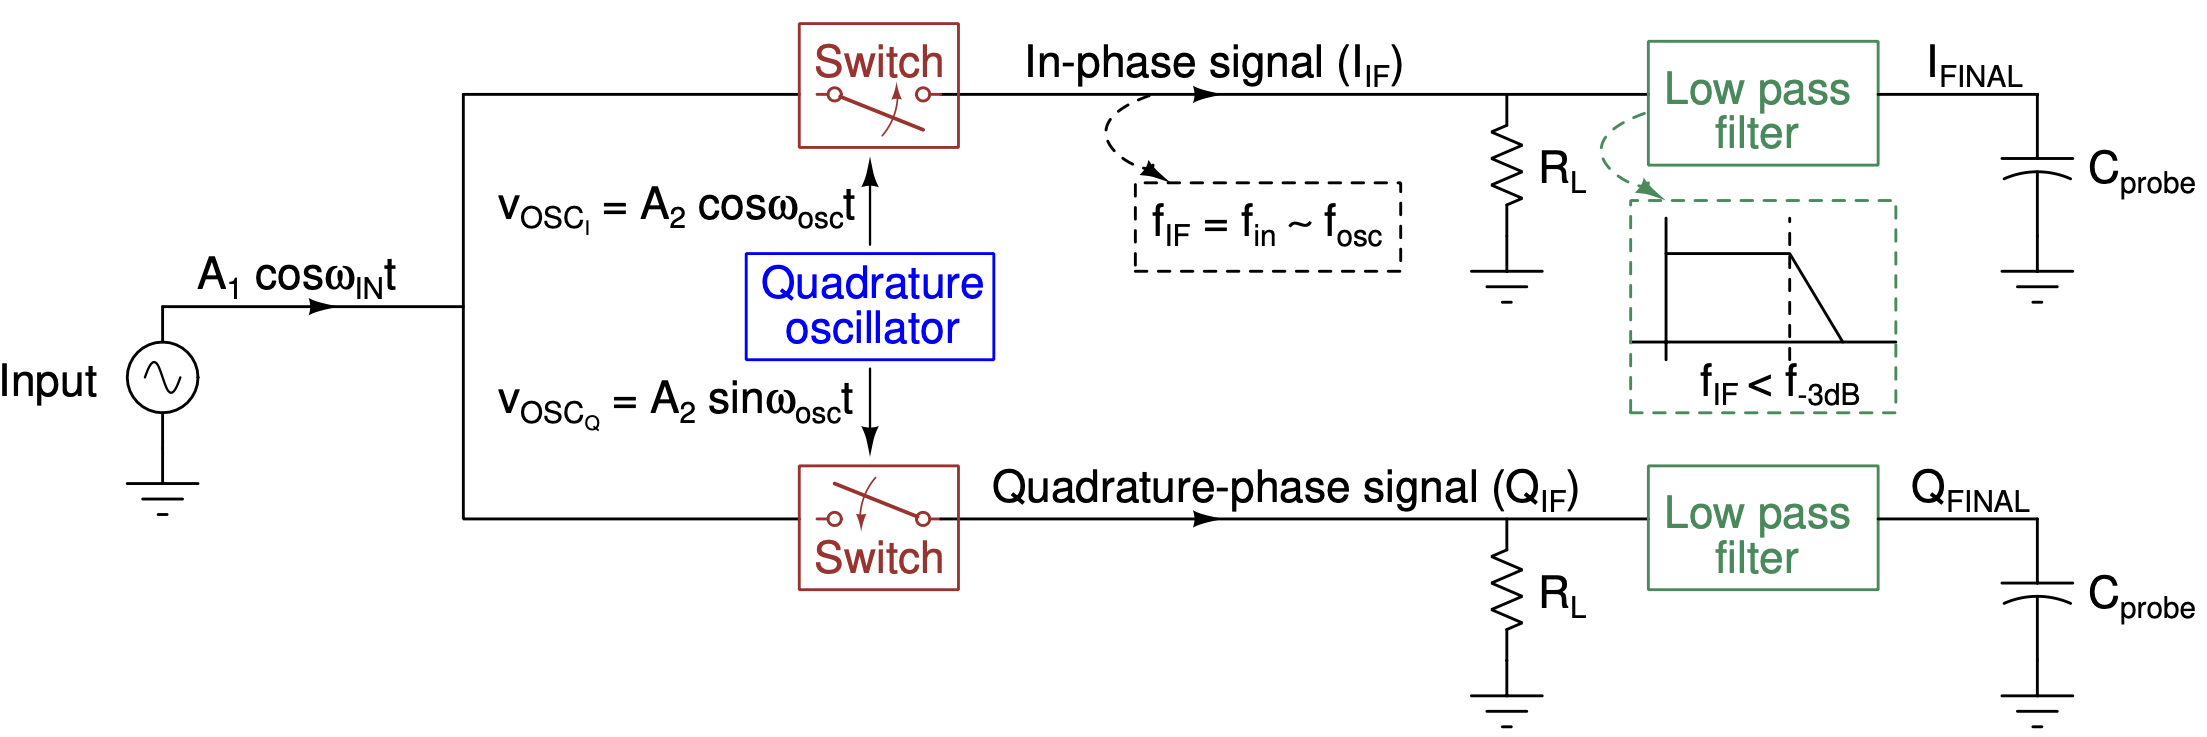
\includegraphics[width=0.5\textwidth, height=4.5cm, keepaspectratio=false]{fig1.png}
    \caption{Circuit Block Diagram}
\end{figure}
\vspace{-0.5cm}
\begin{align}
A \cos(\omega_{IF} t) &= A \cos(\omega_{in} - \omega_{LO}) \tag{i} \\
A \cos(\omega_{IF} t) &= A \cos(\omega_{LO} - \omega_{in}) \tag{ii}
\end{align}



\begin{figure}[htbp]
    \centering
    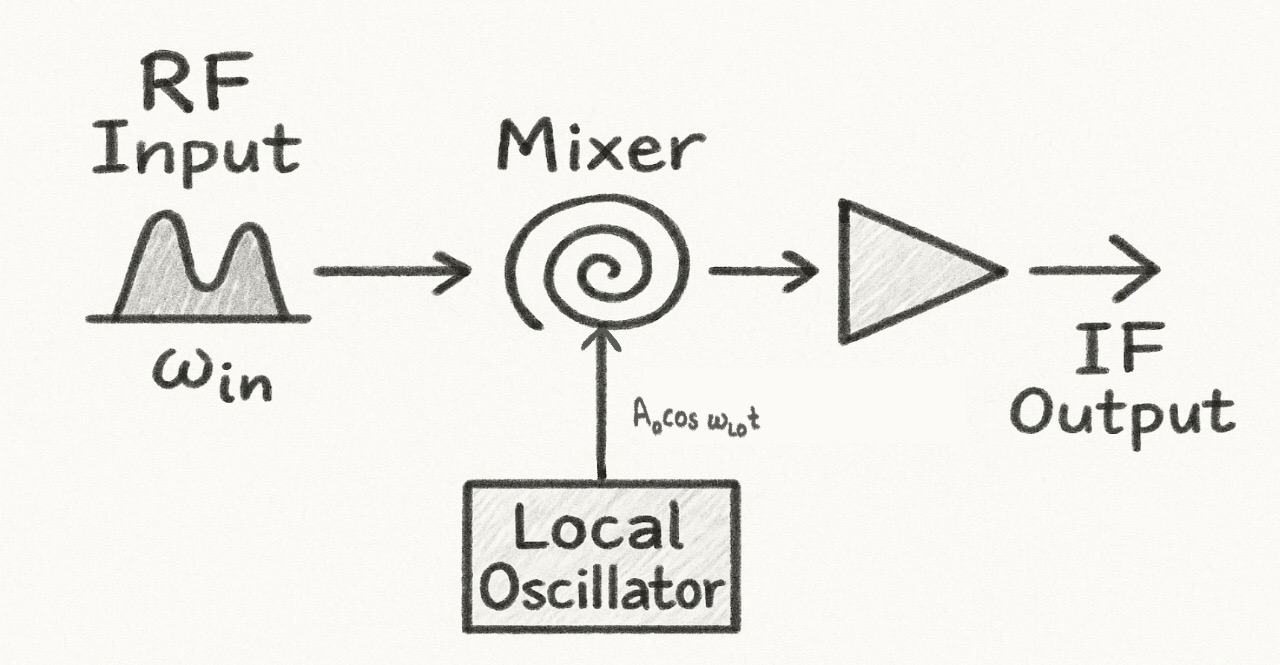
\includegraphics[width=0.5\textwidth, height=5cm, keepaspectratio=false]{fig2.jpeg}
    \caption{Flow Diagram}
\end{figure}

When an asymmetrically modulated signal is down-converted to a zero IF, it can distort unless baseband signals are distinguished by phase. This is addressed by the Quadrature Down Converter (QDC), which generates two versions of the down-converted signal with a 90° phase difference.

In quadrature down conversion, two mixers are used: one with a cosine wave and the other with a sine wave. This splits the RF signal into two paths to produce quadrature baseband signals. The input signal $v_{in} = A_1 \cos(\omega_{in} t)$ mixes with $v_{OSC_I} = A_2 \cos(\omega_{OSC} t)$ and $v_{OSC_Q} = A_2 \sin(\omega_{OSC} t)$, resulting in in-phase ($v_{IFI}$) and quadrature-phase ($v_{IFQ}$) IF signals. These signals maintain a 90° phase difference. The mixed signal is passed through a low-pass filter to retain the IF signals with frequency $\omega_{IF} = (\omega_{in} - \omega_{OSC})$, which is sufficiently low for high $\omega_{in}$ and $\omega_{OSC}$ values. (Note that here both amplitudes are equal for the sine and cosine waves)

\begin{equation}
\begin{split}
v_{IF_I} &= v_{in} \times v_{OSC_I}\\
&= \frac{A_1 A_2}{2} (\cos (\omega_{in}t - \omega_{OSC}t) + \cos (\omega_{in}t + \omega_{OSC}t))
\end{split}
\tag{iv}
\end{equation}

\vspace{-0.5cm}

\begin{equation}
\begin{split}
v_{IF_Q} &= v_{in} \times v_{OSC_Q}\\
&= \frac{A_1 A_2}{2} (\sin(\omega_{in}t + \omega_{OSC}t) - \sin (\omega_{in}t - \omega_{OSC}t))
\end{split}
\tag{v}
\end{equation}

\section{Quadrature Oscillator Design}
Quadrature oscillators are a type of phase-shift sinusoidal oscillator used to generate two sinusoidal signals of equal frequency and amplitude but with a 90\textdegree\ phase difference. These oscillators serve as crucial signal sources in applications such as communications, instrumentation, and digital signal processing. In this lab, we designed a quadrature oscillator using op-amps to generate two outputs—$v_{\text{OSC\_I}} \quad \text{and} \quad v_{\text{OSC\_Q}}$—each with a peak-to-peak amplitude of 1V and a frequency of 100kHz, separated by a 90\textdegree\ phase shift.

\subsection{Concept of Oscillators and Classification}
Oscillators are fundamental circuits that generate periodic waveforms without requiring an external input signal. Quadrature oscillators produce two sinusoidal signals with a fixed 90\textdegree\ phase difference.

The principle of oscillation lies in the feedback loop behavior. When the feedback system becomes unstable due to this condition, the output signal grows until it is limited by the supply rails, forming a stable oscillation.

In the implemented design, a Wien bridge oscillator was used to generate a stable sinusoidal waveform. The Wien bridge oscillator is a topology for low-distortion sine wave generation and consists of an operational amplifier with a frequency-selective feedback network. The bridge network sets the oscillation frequency, while the amplifier provides the necessary gain to satisfy the loop gain condition. Once started, the oscillator produces a clean sine wave at a fixed frequency determined by the RC components in the feedback path.

To obtain the corresponding cosine waveform—which is a 90° phase-shifted version of the sine signal—an integrator circuit was employed. The key principle exploited here is that the integral of a sine wave is a negative cosine wave:
\begin{figure}[h!]
    \centering
    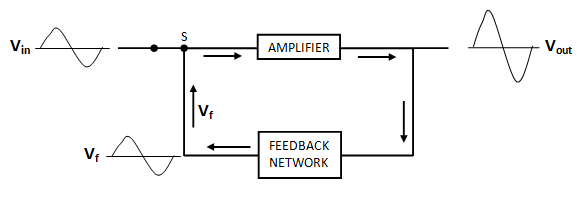
\includegraphics[width=0.5\textwidth]{fig12.png}
    \caption{Basic oscillator feedback circuit}
\end{figure}

\subsection{Structure and Operation of our Quadrature Oscillator}
By feeding the output of the Wien bridge oscillator (the sine wave) into an active integrator (built using an op-amp integrator circuit), the circuit effectively generates the cosine component, with appropriate amplitude scaling and sign inversion. This method ensures that the two resulting waveforms are not only sinusoidal but also exhibit the required 90° phase difference, thereby fulfilling the criteria for quadrature signal generation.
\[
\int \sin(\omega t) \, dt = -\frac{1}{\omega} \cos(\omega t)
\]

This approach simplifies the quadrature oscillator design by separating the generation and phase-shifting tasks: the Wien bridge oscillator ensures stable sinusoidal output, and the integrator circuit accurately produces the quadrature component. This method provides clean, matched-phase signals suitable for applications such as vector modulation, digital communications, and signal processing systems.


The slew rate must be greater than \( 2\pi \, V_P f_o \), where \( V_P \) is the peak voltage and \( f_o \) is the oscillation frequency. Otherwise, distortion of the output signal occurs.

\[
\Phi = \tan^{-1}(-\omega RC) - \tan^{-1}\left(\frac{1}{\omega RC}\right) + \frac{\pi}{2}
\]

\[
\text{Frequency} = \frac{1}{2\pi RC}
\]

\[
\omega = \frac{1}{RC}
\]

\[
\omega = 2\pi f
\]

Oscillation occurs when the overall phase shift around the feedback loop approaches 180\textdegree\, and the magnitude of the loop gain, 
\[
\lvert A\beta \rvert \to 1.
\]
In this condition, the system becomes unstable, and the output voltage starts increasing. However, the power supply limits this growth, preventing the voltage from reaching infinity. As the output approaches either of the supply rails, the value of \( A \) changes slightly, pushing \( A\beta \) away from the unstable point. This causes the voltage rise to slow down and eventually reverse direction. The system then swings toward the opposite rail, and this repeating behavior generates a sinusoidal waveform.

When using large feedback resistors in the design, their interaction with the op-amp’s input capacitance can introduce unwanted poles and zeros in the system. These effects may shift the phase near the oscillation frequency and interfere with stable operation. Additionally, the op-amp's slew rate must be considered. It must be greater than
\[
\text{Slew Rate} > 2\pi V_P f_o,
\]
where \( V_P \) is the peak voltage and \( f_o \) is the desired oscillation frequency. If the slew rate is too low, the waveform will become distorted.

For a quadrature oscillator, oscillation occurs when the frequency satisfies
\[
f = \frac{1}{2\pi RC},
\]
which corresponds to
\[
\omega = \frac{1}{RC},
\]
where the loop gain simplifies to
\[
A\beta = 1 \angle -180^\circ,
\]
allowing sustained oscillations. Increasing the amplifier gain can raise the output amplitude, though it may reduce the overall bandwidth of the system.

\subsection{LTSpice Simulations}

\begin{figure}[H]
    \centering
    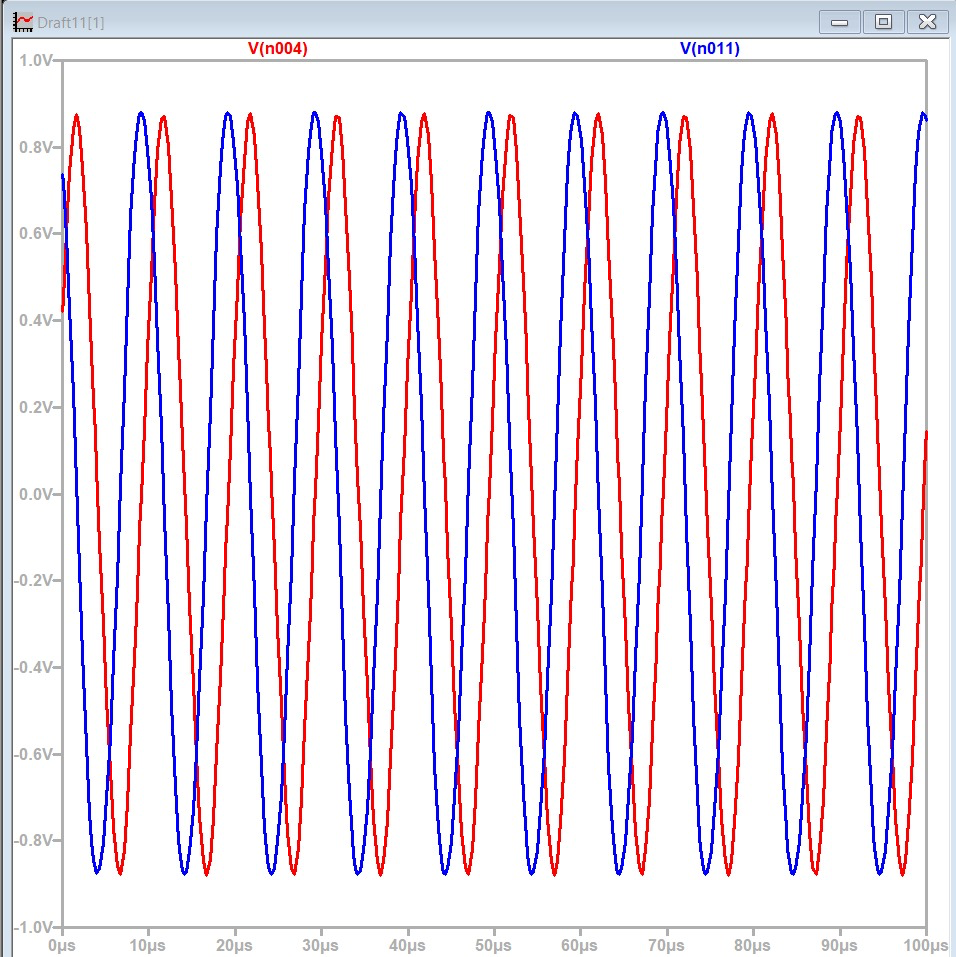
\includegraphics[width=0.4\textwidth, height=6cm, keepaspectratio=false]{oscillator1.png}
    \caption{Output wave form from the oscillator}
\end{figure}

\begin{figure}[H]
    \centering
    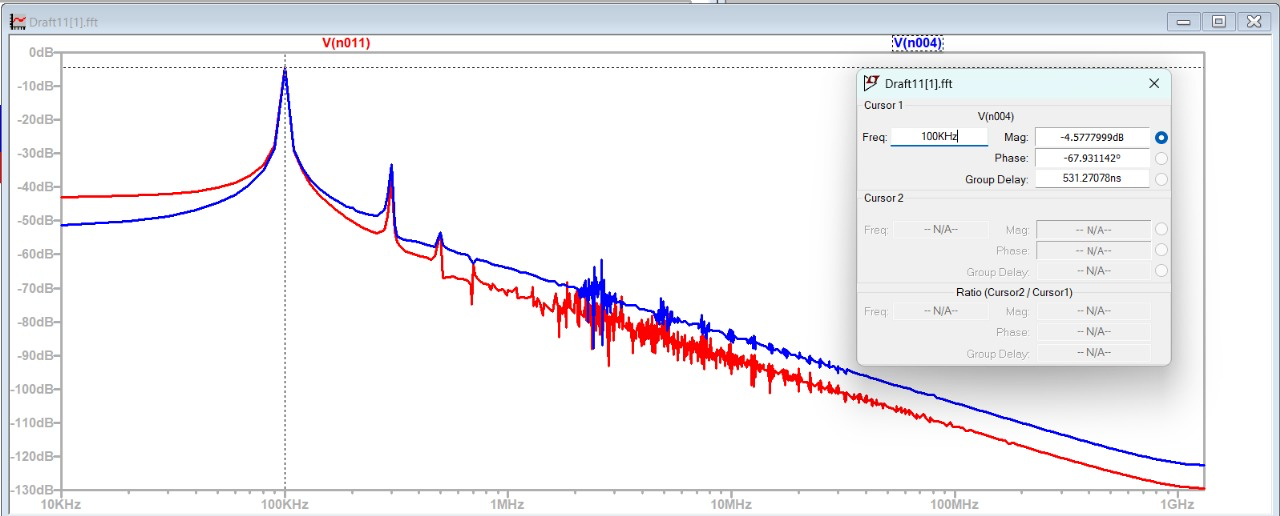
\includegraphics[width=0.4\textwidth, height=6cm, keepaspectratio=false]{oscillator2.png}
    \caption{FFT of the sine wave and its counterpart}
\end{figure}
Notice that the test output is of 100Khz and hence the corresponding highest peak

\begin{figure}[H]
    \centering
    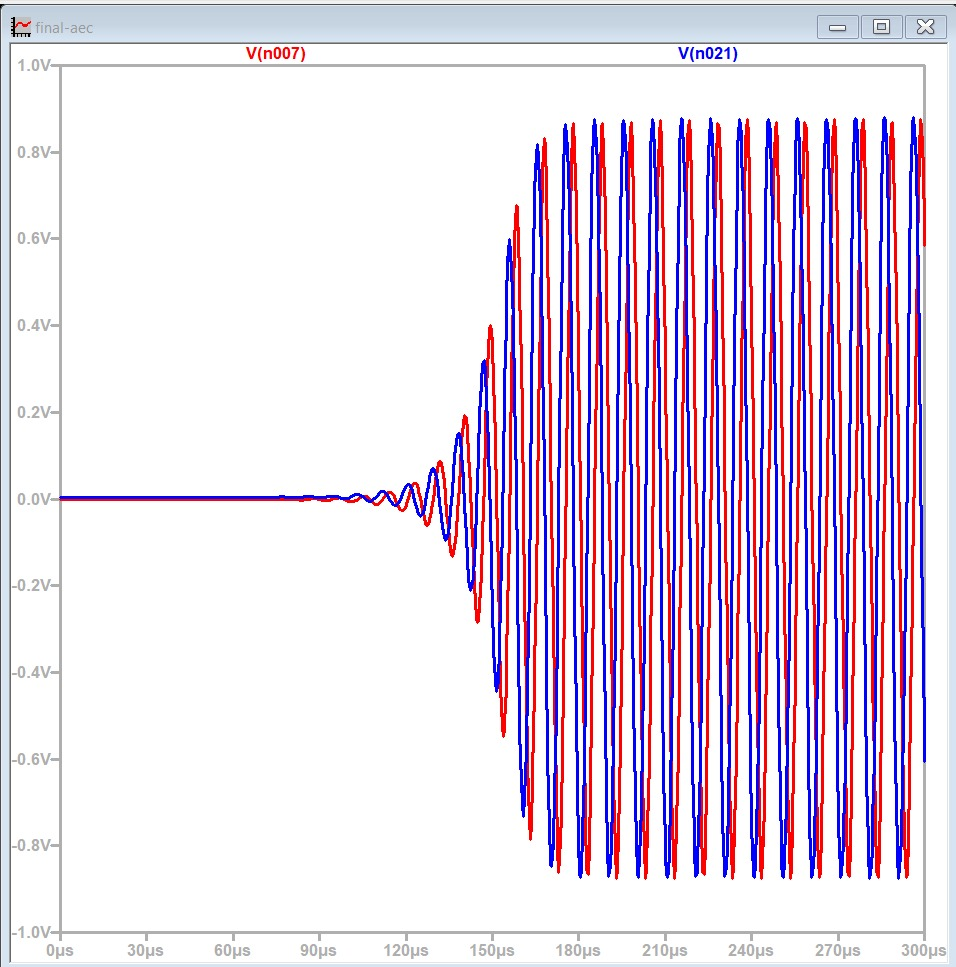
\includegraphics[width=0.4\textwidth, height=6cm, keepaspectratio=false]{bb.jpg}
    \caption{Sine wave and its counterpart}
\end{figure}

\section{Switch(mixer) Design}
A Switch is a device that toggles between (ON) and (OFF) state repeatedly and by doing so, it reaches an approximate multiplication of its two input waveforms.
Here, we have used a mosfet which switches between triode and cutoff mode based upon the oscillatory voltage input given to its gate terminal and a bias voltage which nearly equals its threshold voltage.We do not partake in the sturation region as it is non-linear towards the (gate-source) voltage.
As shown in Fig. 3 (given below), a simple MOSFET can function effectively as a switch (or mixer), where the oscillator signal is applied to the Gate of the MOSFET, the input signal is fed at the Source terminal, and the intermediate frequency (IF) output is extracted from the Drain. This section outlines the principles and design considerations for achieving an ideal switch using a MOSFET, including the requirements for minimizing internal resistance and achieving a 50\% duty cycle.
Duty Cycle refers to the ratio of the time it is switched on and the total time. It indicates us to the extent or the division of time between on and off modes.

\begin{figure}[htbp]
    \centering
    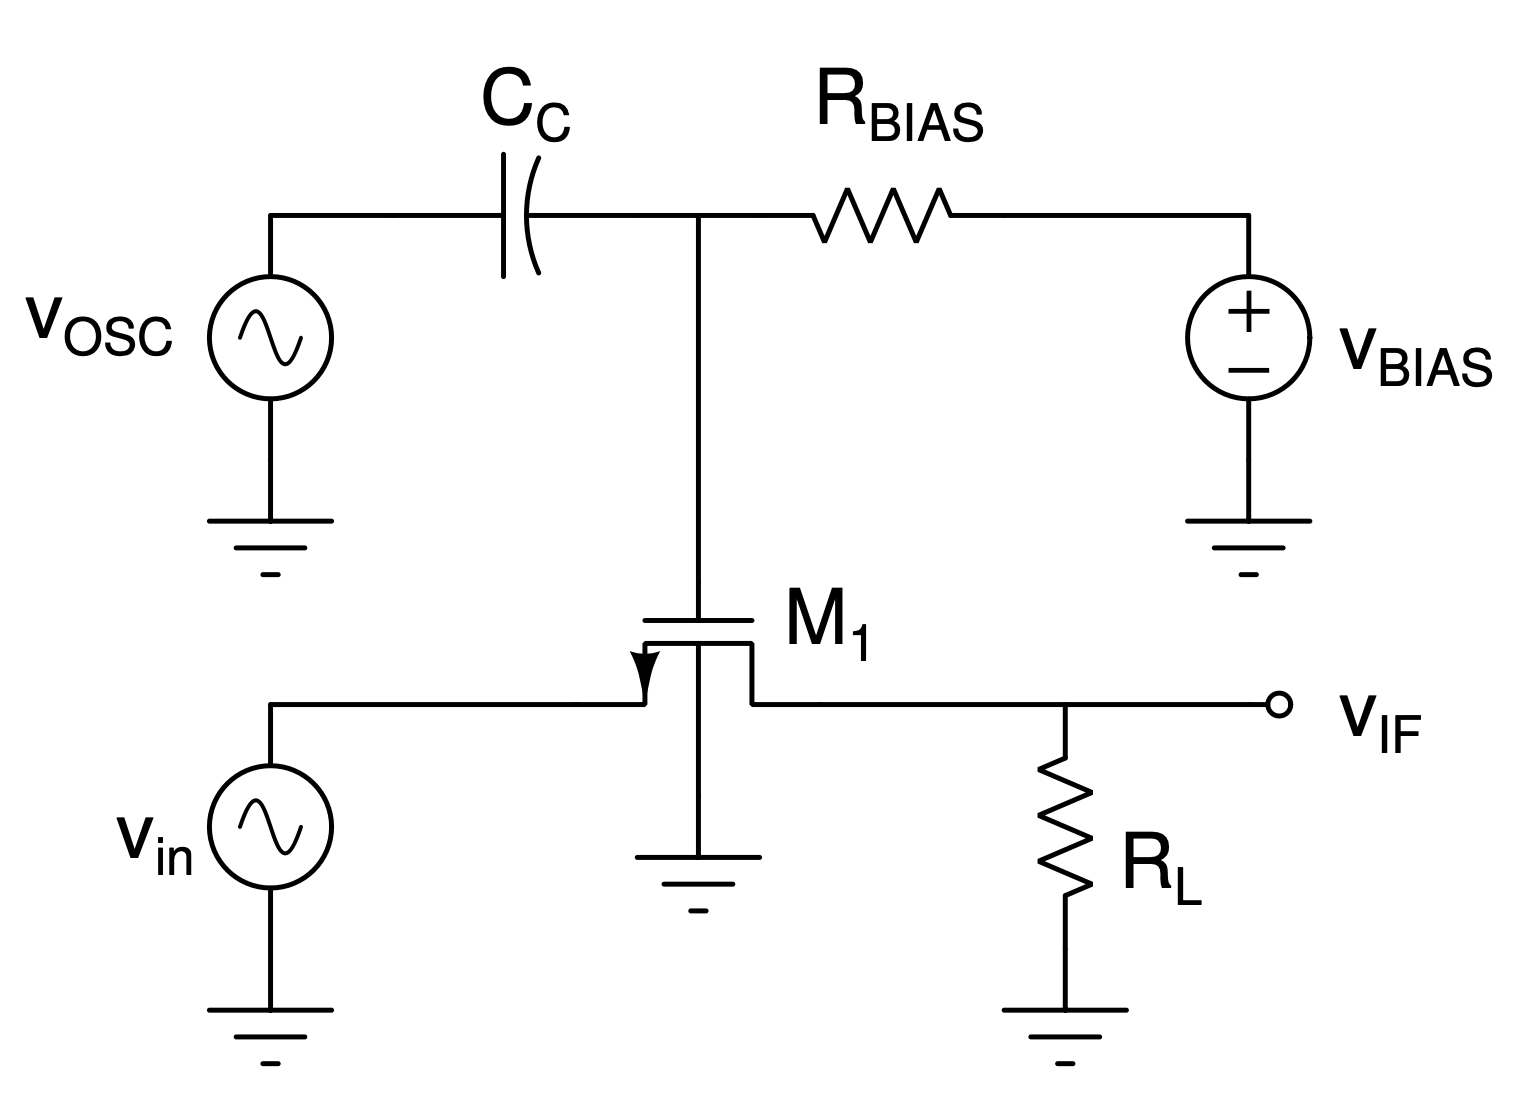
\includegraphics[width=0.5\textwidth, height=6cm, keepaspectratio=false]{fig3.png}
    \caption{Circuit Diagram for Mixer}
\end{figure}

\subsection{Conditions for an Ideal Switch}

To approach ideal switch behavior, two major conditions must be satisfied:

\begin{itemize}
    \item Duty cycle: The switch should ideally operate with a duty cycle close to 50\%.
    \item Internal resistance: The internal resistance of the switch should be as low as possible, ideally approaching zero.
\end{itemize}

These requirements can be met using a simple MOSFET configuration. In such a setup, the oscillator signal is directed to the gate terminal of the MOSFET, the input signal is applied to the source, and the resulting intermediate frequency signal is obtained from the drain.

\subsection{Achieving low Internal Resistance}

A MOSFET behaves like a linear resistor when operated in the linear or triode region. This behavior allows it to be used as a switch. The drain current in this region is given by:

\[
I_D = \mu_n C_{ox} \frac{W}{L} \left[(V_{GS} - V_{TH})V_{DS} - \frac{V_{DS}^2}{2} \right]
\]

When \( V_{DS} <  2(V_{GS} - V_{TH}) \), this simplifies to:

\[
I_D \approx \mu_n C_{ox} \frac{W}{L}(V_{GS} - V_{TH})V_{DS}
\]

This region is referred to as the deep triode region. In this region, the drain current is a linear function of \( V_{DS} \). For small values of \( V_{DS} \), each I-V parabola can be approximated by a straight line. This linear relationship implies that the path from source to drain can be modeled as a linear resistor, with resistance given by:

\[
R_{ON} = \frac{1}{\mu_n C_{ox} \frac{W}{L}(V_{GS} - V_{TH})}
\]

To make the switch more ideal, this resistance must be minimized. Since the technological parameters such as \( \mu_n \), \( C_{ox} \), and \( V_{TH} \) are fixed for a given process, the only controllable factor is the aspect ratio \( \frac{W}{L} \). Increasing this ratio results in lower on-resistance. The trade off here is bandwidth and the output swing. Due to the increase in the aspect ratio \( \frac{W}{L} \), intrisnic capacitances of the mosfet increase along with its gain. This decreases the output bandwidth and the output swing. Hence a balance of both worlds is necessary.

\begin{figure}[htbp]
    \centering
    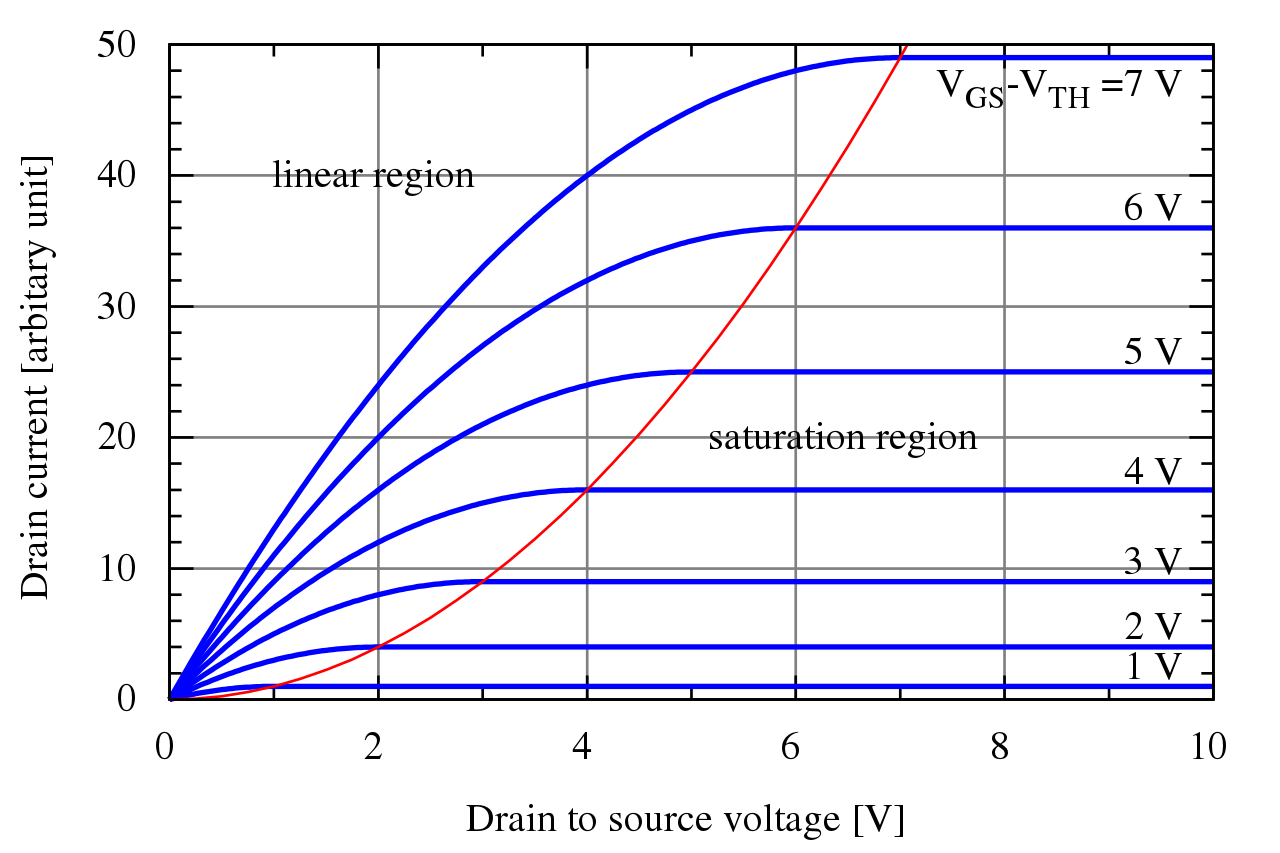
\includegraphics[width=0.5\textwidth, height=6cm, keepaspectratio=false]{fig4.png}
    \caption{$V_{DS}$ vs $I_{D}$ characteristics}
\end{figure}

\subsection{Achieving 50\% Duty Cycle}
A 50\% duty cycle is necessary to make sure the output signal is a close approximation of the multiplied input signals. With changes in that ratio, the output signal is affected and hence will result in an inaccurate multiplication.
To ensure a 50\% duty cycle for switching, the gate voltage \( V_G \) must swing symmetrically around the threshold voltage \( V_{TH} \). This means that the oscillator signal \( V_{osc} \) must be centered around \( V_{TH} \), as the NMOS transistor conducts when \( V_{GS} > V_{TH} \) and remains off when \( V_{GS} < V_{TH} \).

However, implementing this biasing is not straightforward due to the following challenge:

The gate presents a high impedance, and an AC signal tends to seek a low-impedance path to ground. Connecting both AC and DC sources directly to the gate is problematic because the low internal resistance of an ideal source causes the AC current to preferentially flow through the DC source. Similarly, DC current could improperly flow into the AC source.

To resolve this, we introduce biasing components:

\begin{itemize}
    \item A capacitor \( C_{BIAS} \) is placed next to the AC source to block DC current from flowing through it.
    \item A resistor \( R_{BIAS} \) is placed next to the DC source to block AC current from flowing into it.
\end{itemize}

This creates a proper DC biasing path for the gate while allowing the oscillator signal to modulate the transistor.

The chosen component values are:
\[
C_{BIAS} = 10\,\mu\text{F}, \quad R_{BIAS} = 1\,\text{M}\Omega
\]

These values ensure that the gate is appropriately biased for switching with minimal interference between the AC and DC paths.

\subsection{LTSpice Simulations}

\begin{figure}[H]
    \centering
    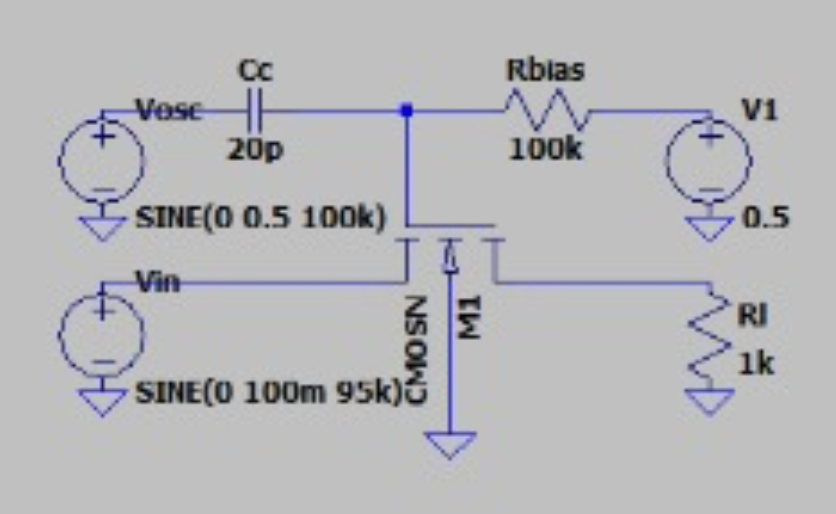
\includegraphics[width=0.45\textwidth]{fig5.png}
    \caption{Mixer Circuit}
\end{figure}

We have taken 
\[
C_{C} = 20p\text{F}
\]
\[
R_{BIAS} = 100\,\text{k}\Omega
\]
\[
R_{L} = 1\,\text{k}\Omega
\]
\[
v_{in} = 100\text{mV}
\]

For different values of \(f_{\text{IN}}\) we get slightly different plots. To observe the effect of increasing \(f_{\text{IN}}\), let us vary \(f_{\text{IN}}\) and observe the plots accordingly.

\clearpage
\textbf{\boldmath\( f_{\text{IN}} = 95\,\text{kHz} \)}
\begin{figure}[H]
    \centering
    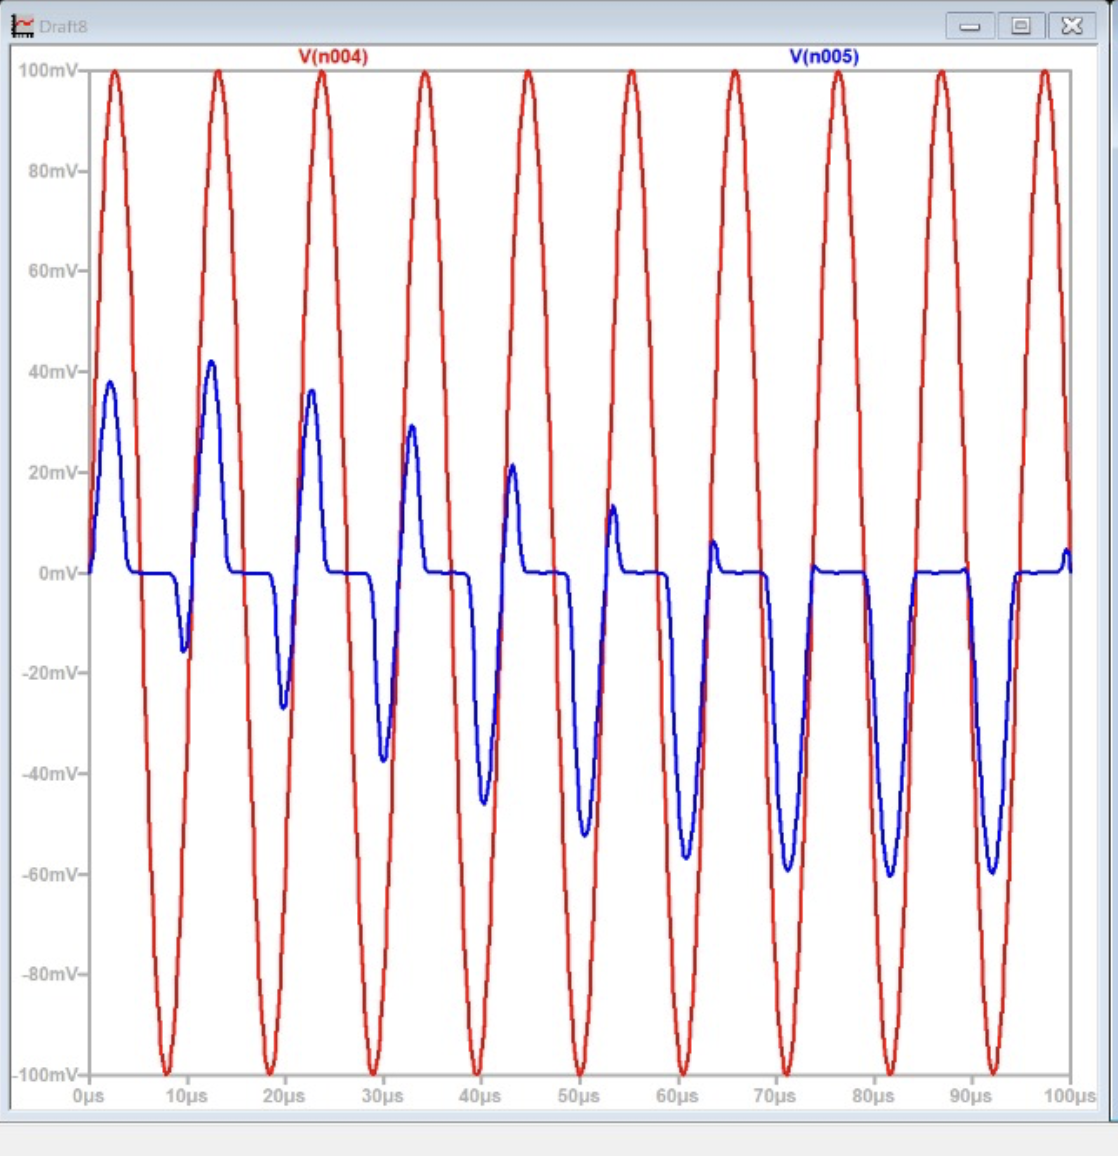
\includegraphics[width=0.3\textwidth]{fig6_95_1.png}
    \caption{(a) \( v_{in} \) vs \( v_{IF} \)}
\end{figure}
\begin{figure}[H]
    \centering
    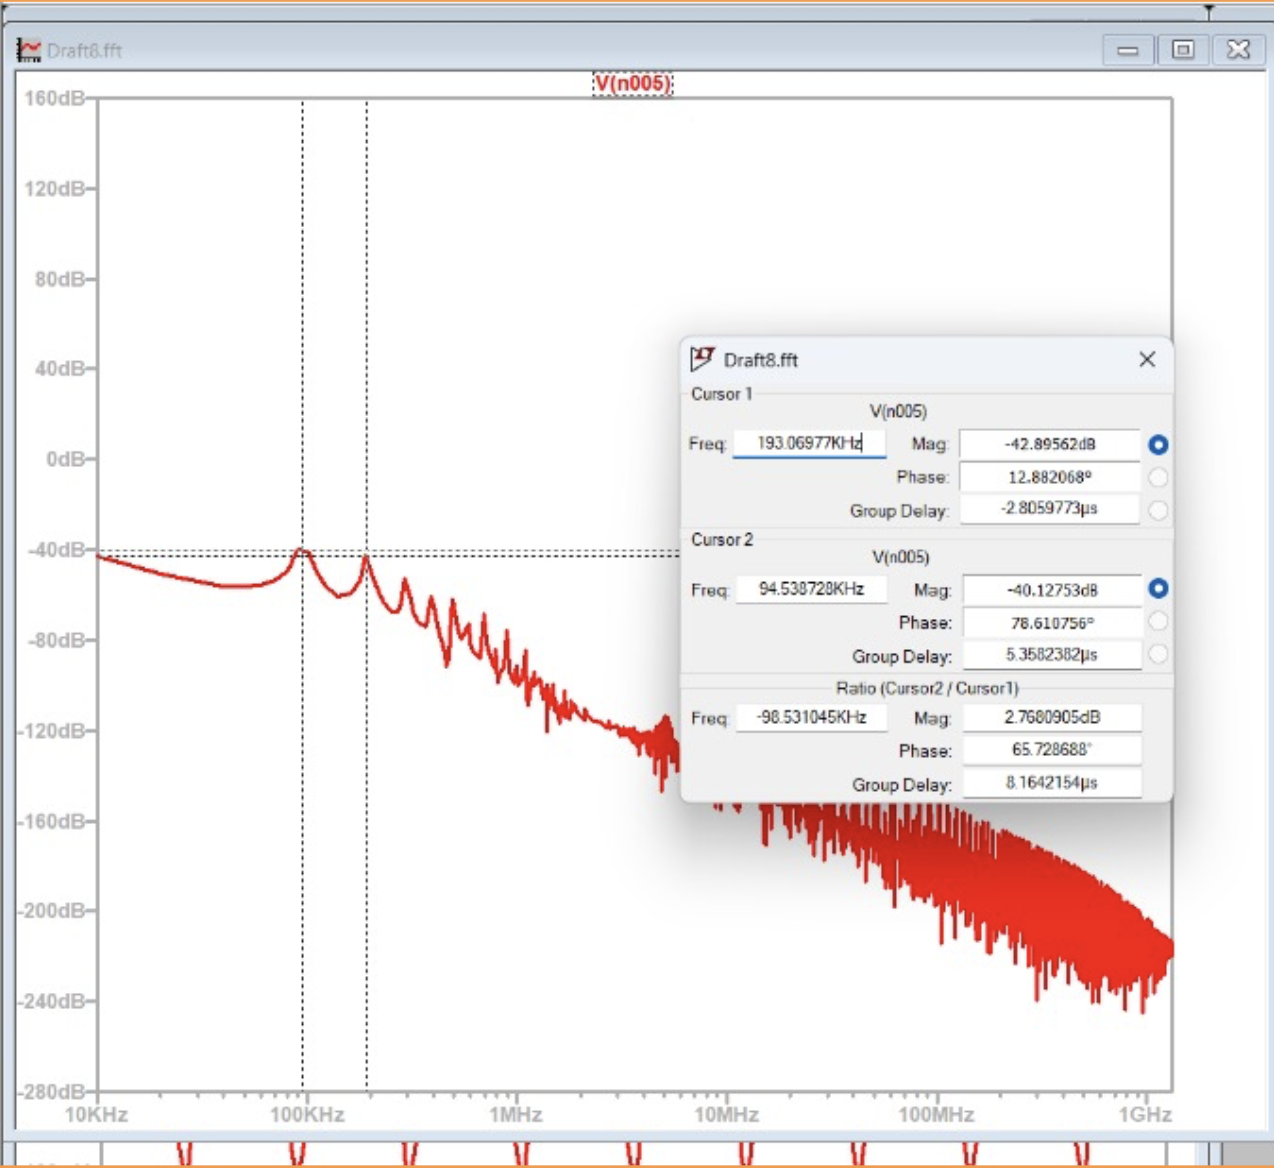
\includegraphics[width=0.4\textwidth]{fig6_95_2.png}
    \caption{(b) fft}
\end{figure}

\textbf{\boldmath\( f_{\text{IN}} = 98\,\text{kHz} \)}
\begin{figure}[H]
    \centering
    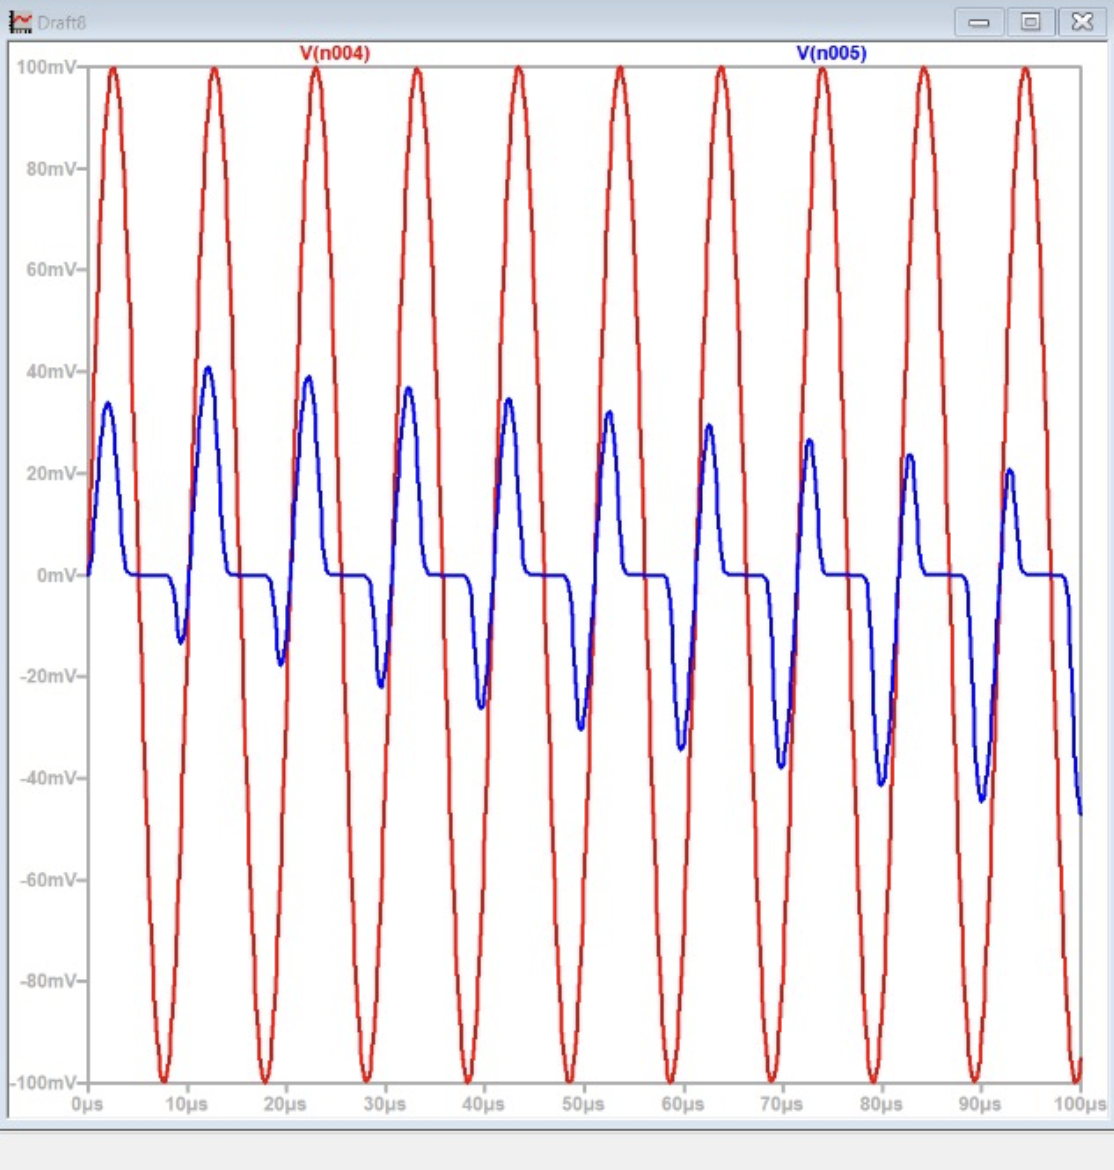
\includegraphics[width=0.3\textwidth]{fig7_98_1.png}
    \caption{(a) \( v_{in} \) vs \( v_{IF} \)}
\end{figure}
\begin{figure}[H]
    \centering
    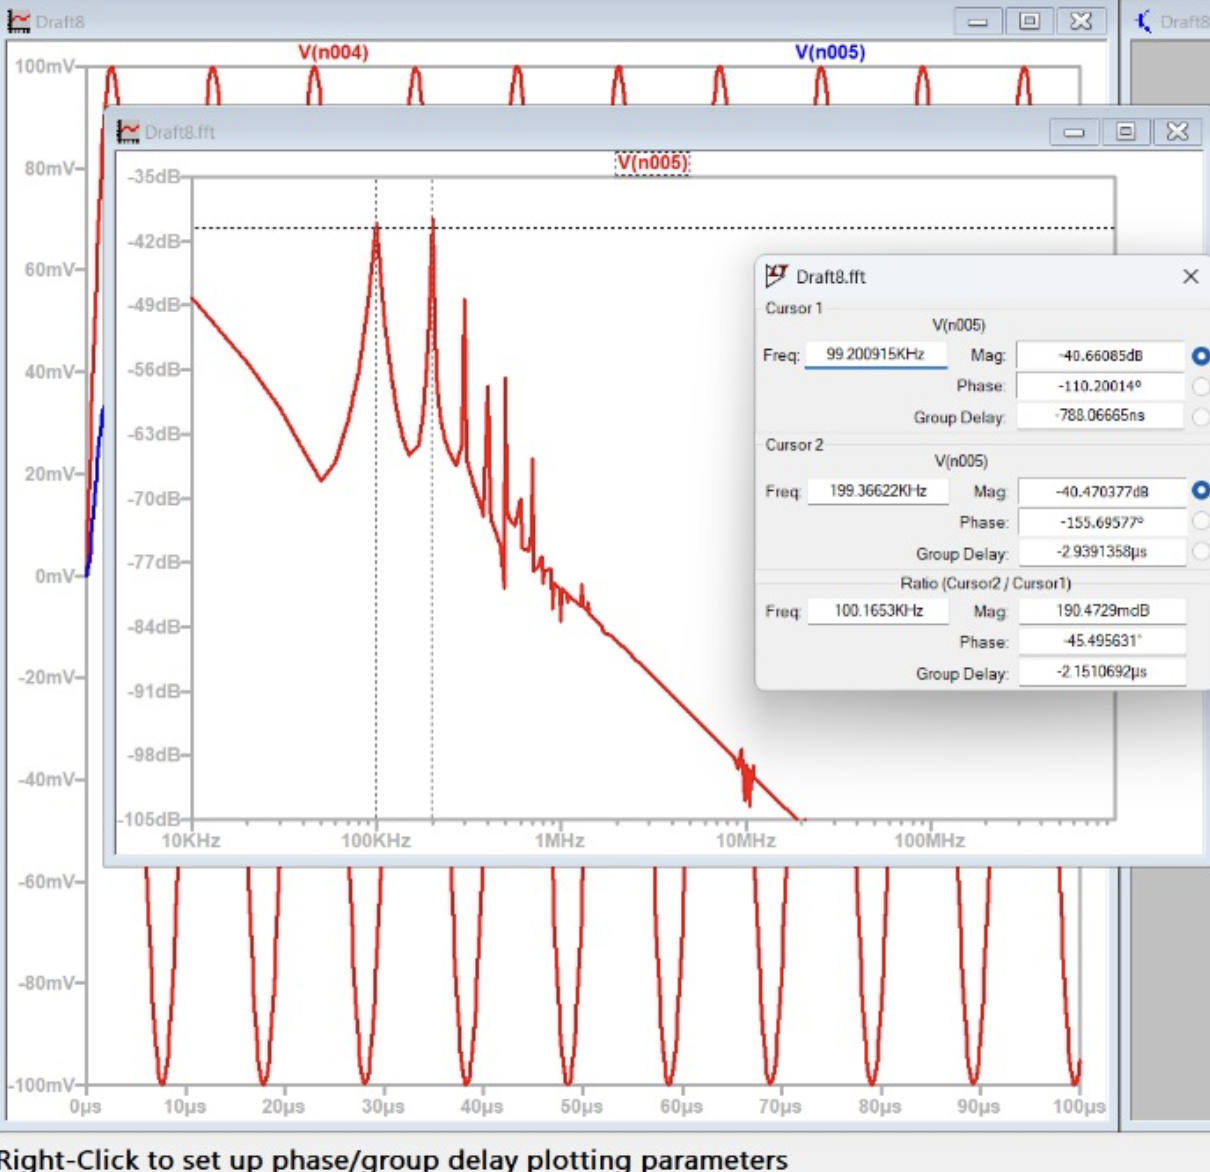
\includegraphics[width=0.4\textwidth]{fig7_98_2.png}
    \caption{(b) fft}
\end{figure}

\textbf{\boldmath\( f_{\text{IN}} = 99\,\text{kHz} \)}
\begin{figure}[H]
    \centering
    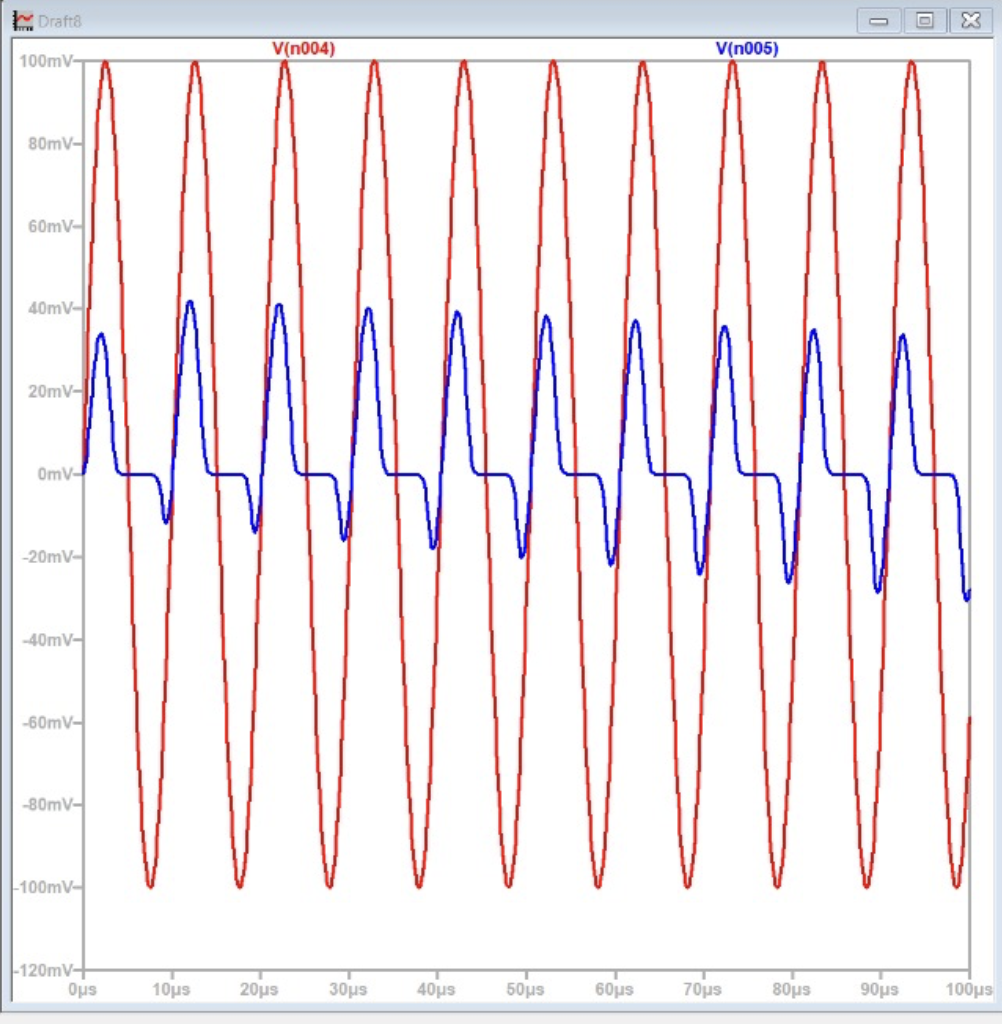
\includegraphics[width=0.3\textwidth]{fig8_99_1.png}
    \caption{(a) \( v_{in} \) vs \( v_{IF} \)}
\end{figure}
\begin{figure}[H]
    \centering
    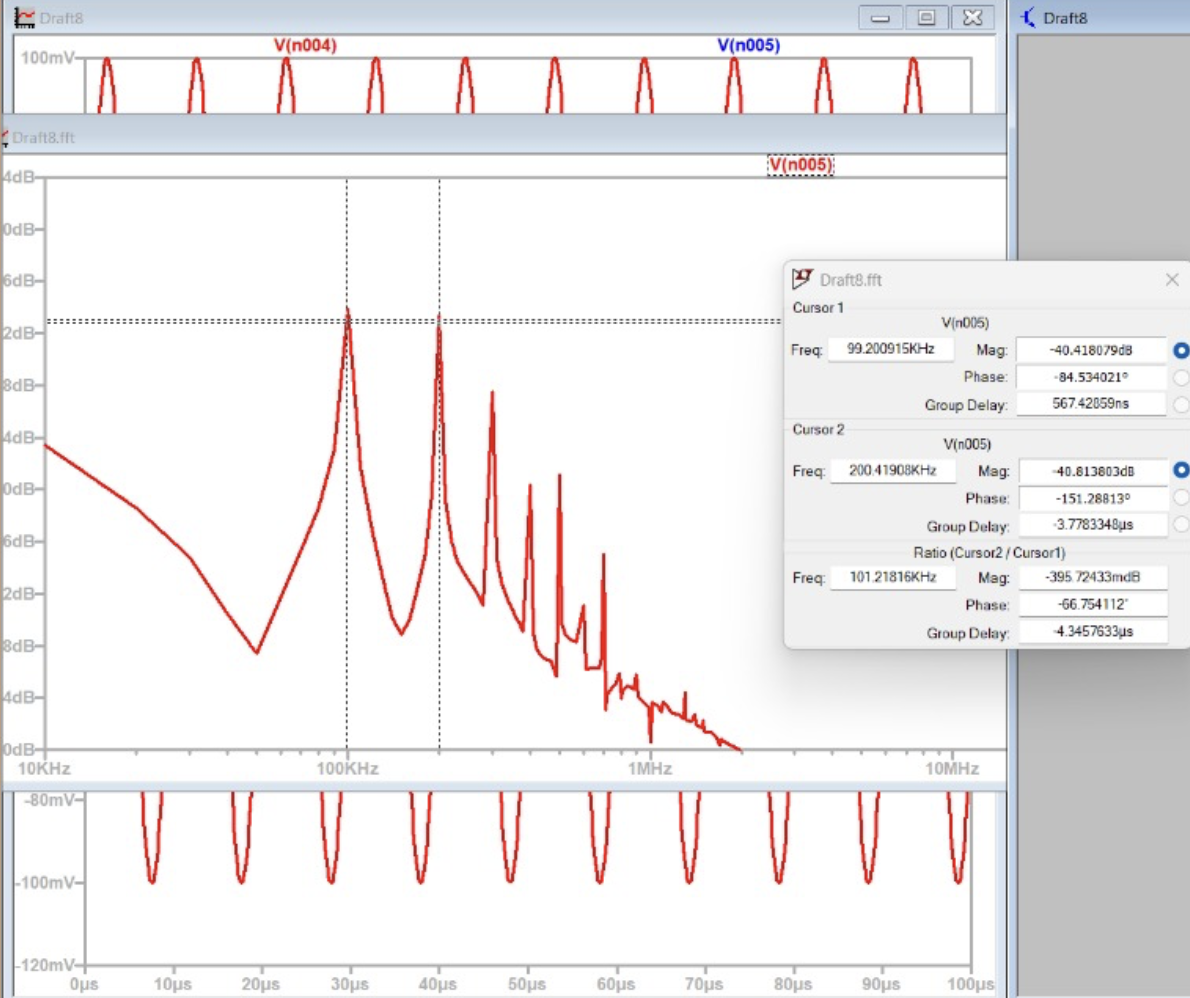
\includegraphics[width=0.45\textwidth]{fig8_99_2.png}
    \caption{(b) fft}
\end{figure}

\textbf{\boldmath\( f_{\text{IN}} = 101\,\text{kHz} \)}
\begin{figure}[H]
    \centering
    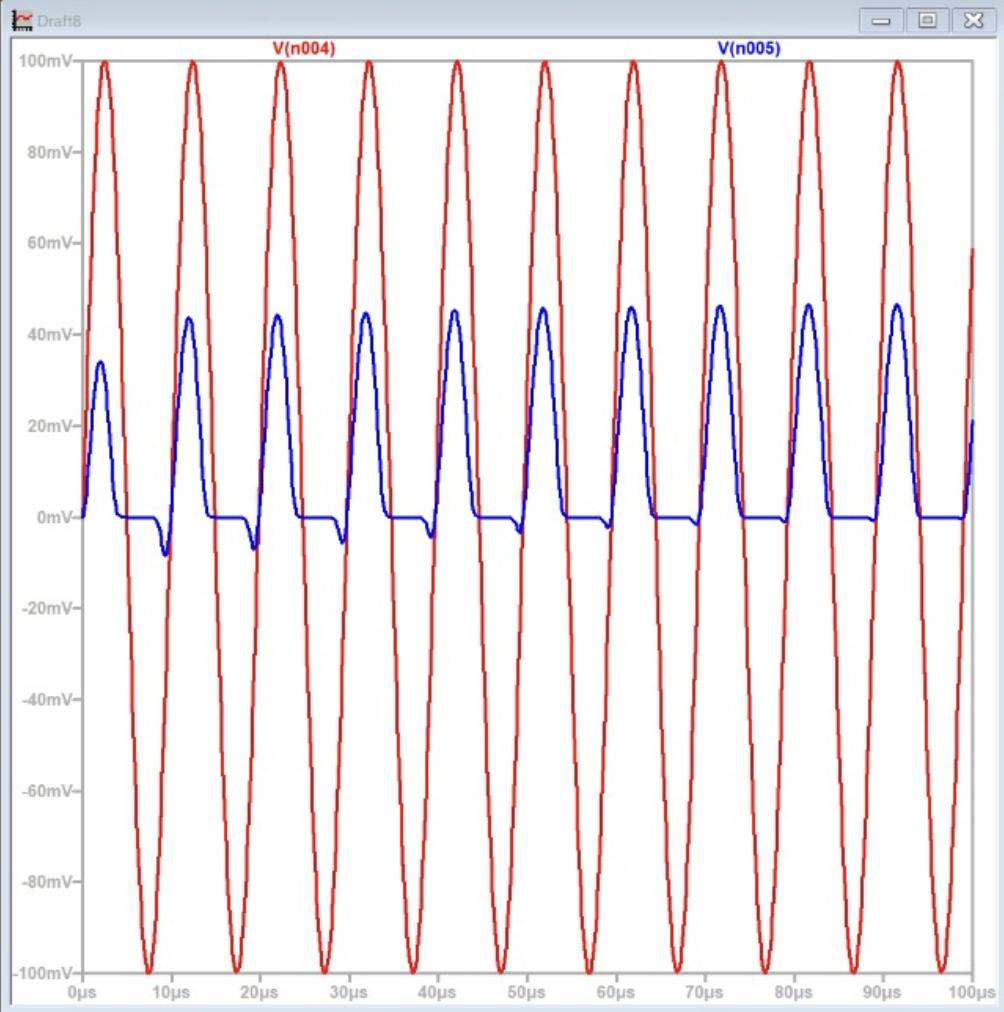
\includegraphics[width=0.3\textwidth]{fig9_101_1.png}
    \caption{(a) \( v_{in} \) vs \( v_{IF} \)}
\end{figure}
\begin{figure}[H]
    \centering
    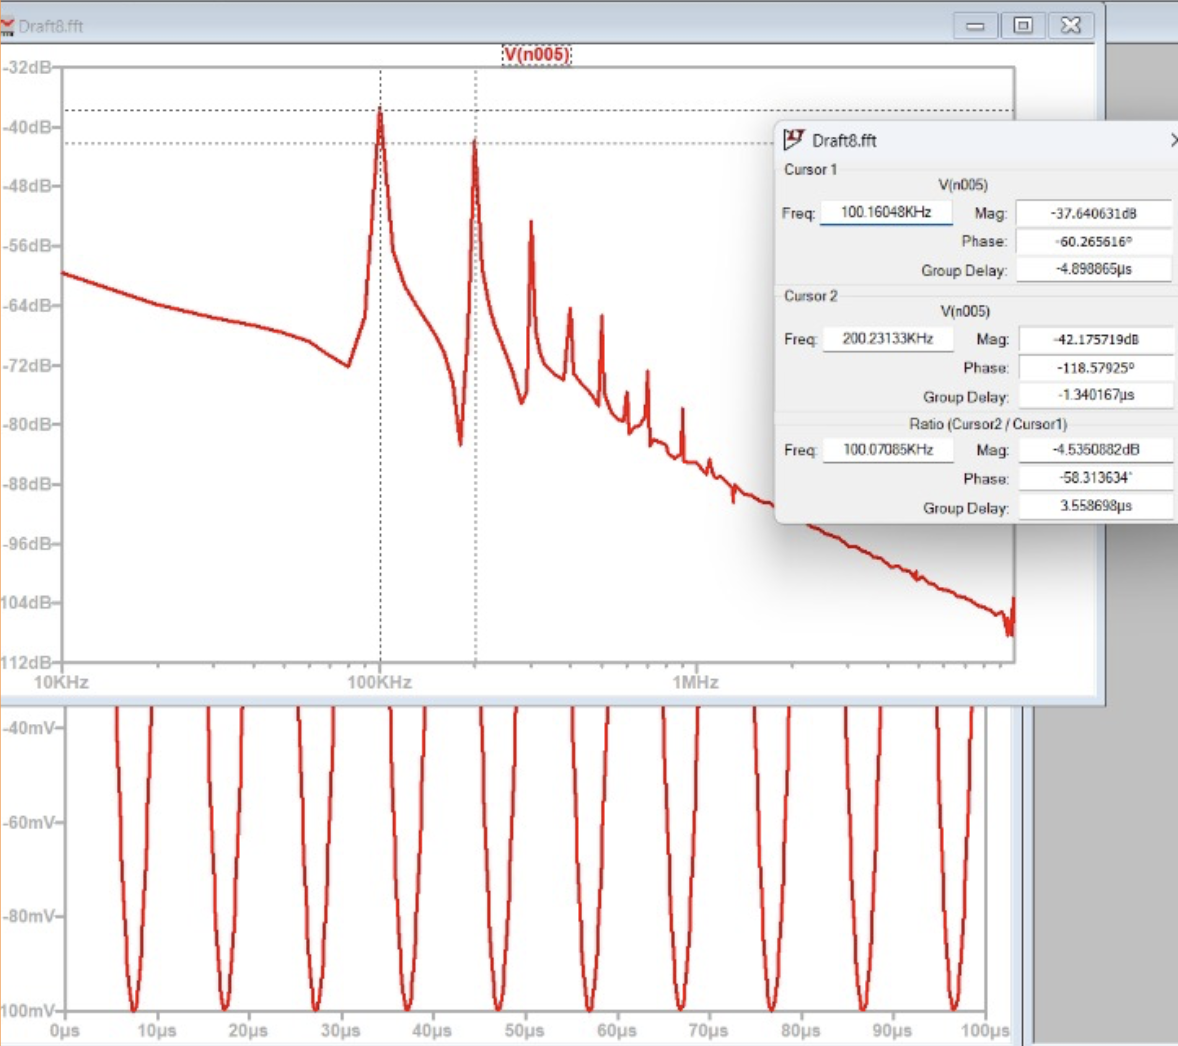
\includegraphics[width=0.45\textwidth]{fig9_101_2.png}
    \caption{(b) fft}
\end{figure}

\textbf{\boldmath\( f_{\text{IN}} = 102\,\text{kHz} \)}
\begin{figure}[H]
    \centering
    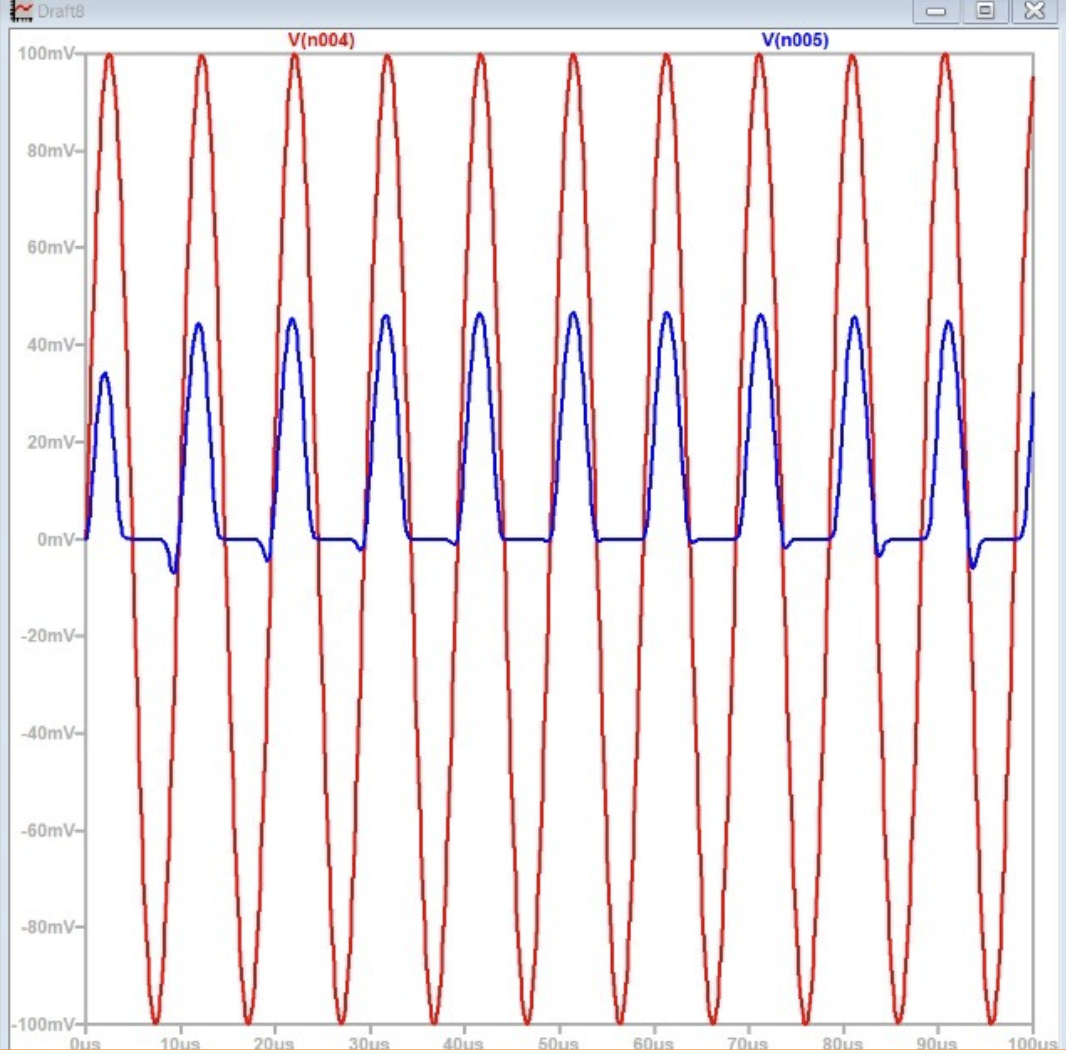
\includegraphics[width=0.3\textwidth]{fig10_102_1.png}
    \caption{(a) \( v_{in} \) vs \( v_{IF} \)}
\end{figure}
\begin{figure}[H]
    \centering
    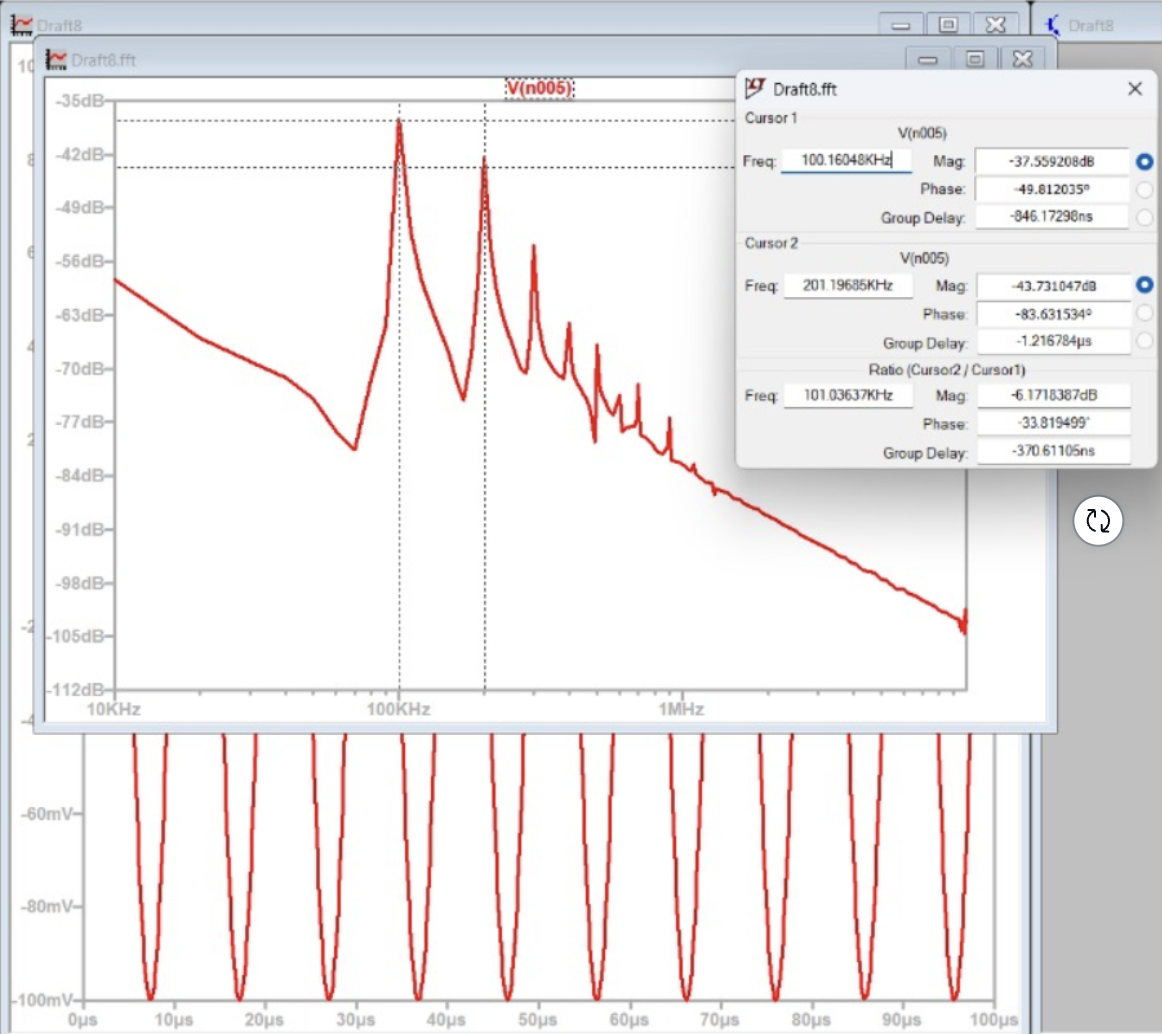
\includegraphics[width=0.4\textwidth]{fig10_102_2.png}
    \caption{(b) fft}
\end{figure}

\textbf{\boldmath\( f_{\text{IN}} = 105\,\text{kHz} \)}
\begin{figure}[H]
    \centering
    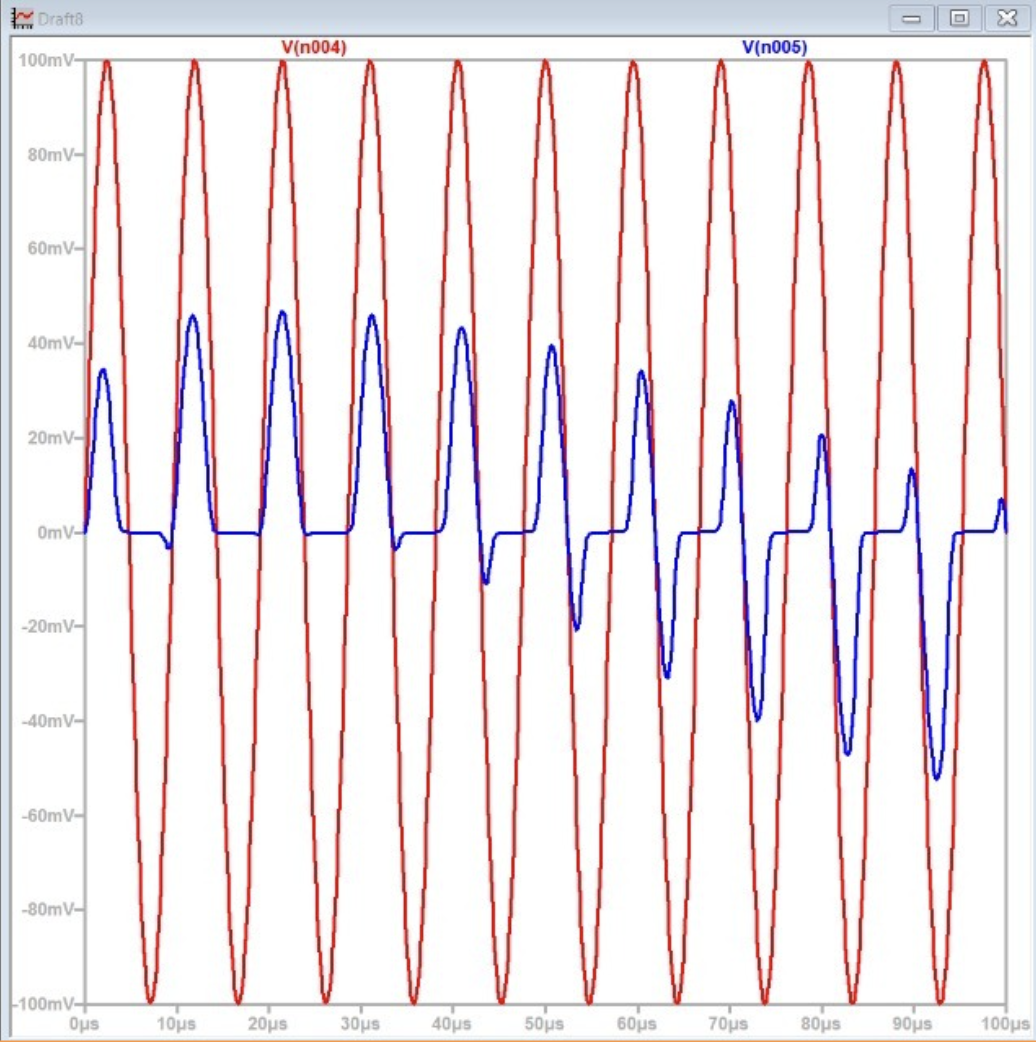
\includegraphics[width=0.3\textwidth]{fig11_105_1.png}
    \caption{(a) \( v_{in} \) vs \( v_{IF} \)}
\end{figure}
\begin{figure}[H]
    \centering
    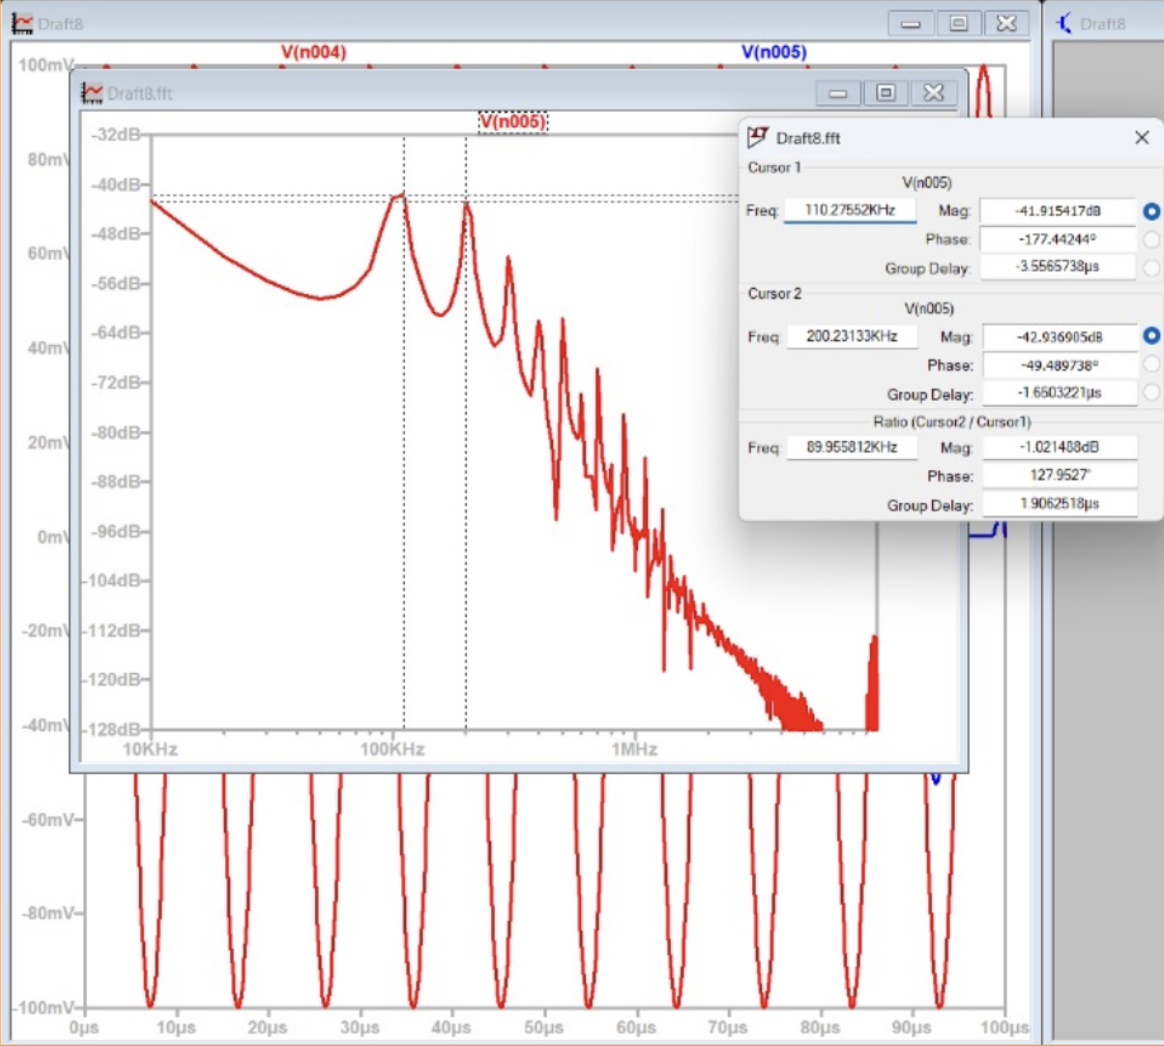
\includegraphics[width=0.4\textwidth]{fig11_105_2.png}
    \caption{(b) fft}
\end{figure}

\section{Low Pass Filter}
A simple low-pass filter can be constructed using a resistor and a capacitor. This type of filter allows low-frequency signals to pass through while attenuating higher-frequency signals. The basic circuit diagram for a low-pass filter using an RC (resistor-capacitor) combination is shown below.

\begin{figure}[H]
    \centering
    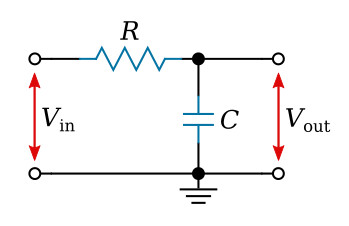
\includegraphics[width=0.4\textwidth]{RC filter.png}
    \caption{RC low pass filter}
\end{figure}

\subsection{Theoretical Derivation}

\subsubsection{Canonical Transfer Function}
The standard second-order low-pass Butterworth filter transfer function is given by:

\begin{equation}
H(s) = \frac{\omega_c^2}{s^2 + \frac{\omega_c}{Q}s + \omega_c^2}
\label{eq:canonical}
\end{equation}

where:
\begin{itemize}
\item $\omega_c = 2\pi f_c$ is the cutoff frequency (12,566 rad/s for 2 kHz)
\item $Q = \frac{1}{\sqrt{2}} \approx 0.7071$ is the quality factor for Butterworth response
\end{itemize}

\subsubsection{Sallen-Key Implementation}
The unity-gain Sallen-Key topology realizes this transfer function as:

\begin{equation}
H(s) = \frac{1}{R_1R_2C_1C_2s^2 + (R_1C_1 + R_2C_1)s + 1}
\label{eq:sallenkey}
\end{equation}

\subsubsection{Coefficient Matching}
Equating coefficients between \eqref{eq:canonical} and \eqref{eq:sallenkey}:

\begin{align}
s^2 &: R_1R_2C_1C_2 = \frac{1}{\omega_c^2} \label{eq:coeff1} \\
s^1 &: R_1C_1 + R_2C_1 = \frac{1}{Q\omega_c} \label{eq:coeff2} \\
s^0 &: 1 = 1 \quad \text{(automatically satisfied)}
\end{align}

\subsubsection{Equal Resistor Simplification}
Setting $R_1 = R_2 = R$ yields:

\begin{equation}
R = \frac{1}{\omega_c\sqrt{C_1C_2}}
\label{eq:Rcalc}
\end{equation}

\begin{equation}
C_2 = \frac{1}{4Q^2C_1} = \frac{1}{4 \times 0.5 \times C_1} = \frac{1}{2C_1}
\label{eq:Cratio}
\end{equation}

\subsection{Theoretical Component Values}

For $f_c = 2$ kHz and selecting $C_1 = 5$ nF:

\begin{align*}
C_2 &= \frac{1}{2 \times 5\text{nF}} = 10\text{nF} \\
R &= \frac{1}{12,566 \times \sqrt{5\text{nF} \times 10\text{nF}}} \\
&= 7.96\text{k}\Omega
\end{align*}

\subsection{Experimental Discrepancies and Corrections}

\subsubsection{Observed Behavior}
Initial implementation with theoretical values showed:
\begin{itemize}[leftmargin=*]
\item Actual cutoff frequency: 1.82 kHz (-9\% error)
\item Passband ripple: 0.8 dB (expected 0 dB for Butterworth)
\end{itemize}

\subsubsection{Empirical Optimization}
Through iterative testing, we found optimal performance with:
\begin{align*}
C_2 &= 5.93\text{nF} \quad \text{(vs theoretical 10nF)} \\
R &= 7.96\text{k}\Omega \quad \text{(unchanged)}
\end{align*}

\subsection{Frequency Response Validation}

Key measurements:
\begin{itemize}
\item -3 dB point: 2.01 kHz (0.5\% error from target)
\item Stopband attenuation: -38 dB/decade (close to ideal -40 dB/decade)
\end{itemize}

\begin{figure}[H]
    \centering
    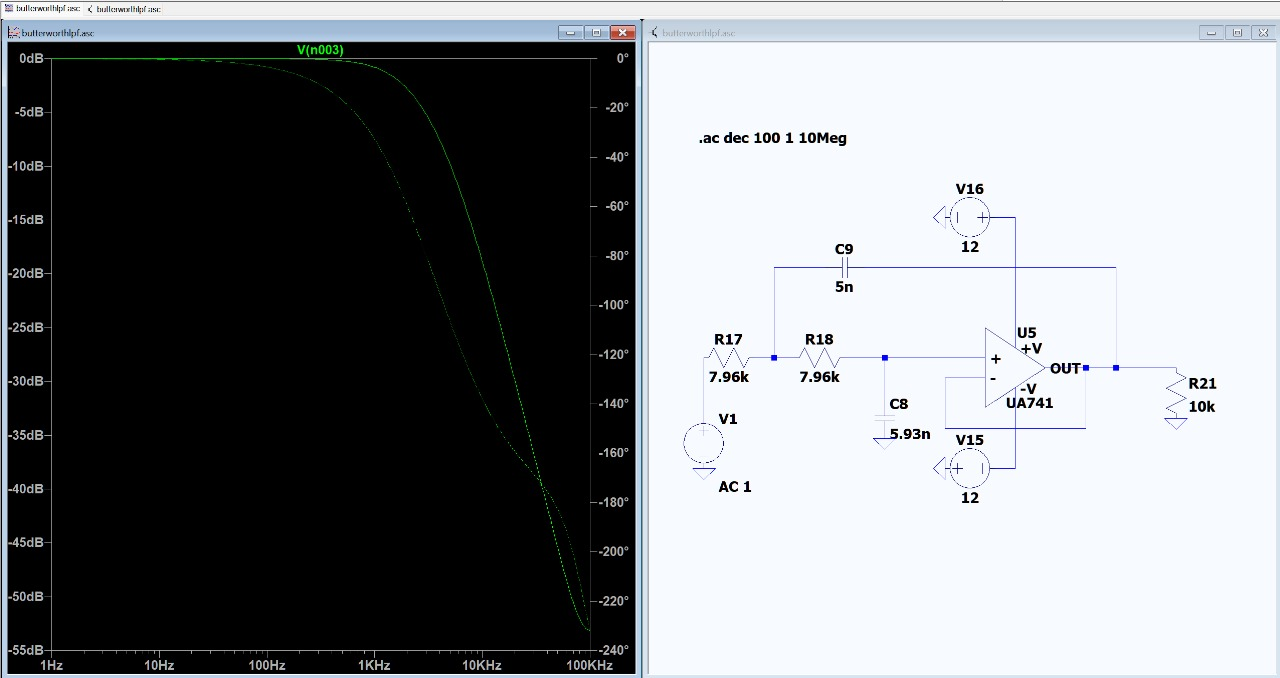
\includegraphics[width=1\linewidth]{WhatsApp Image 2025-05-03 at 22.54.23_3a84ccdd.jpg}
    \caption{Bode plot of the low pass filter}
    \label{fig:enter-label}
\end{figure}
\begin{figure}[H]
    \centering
    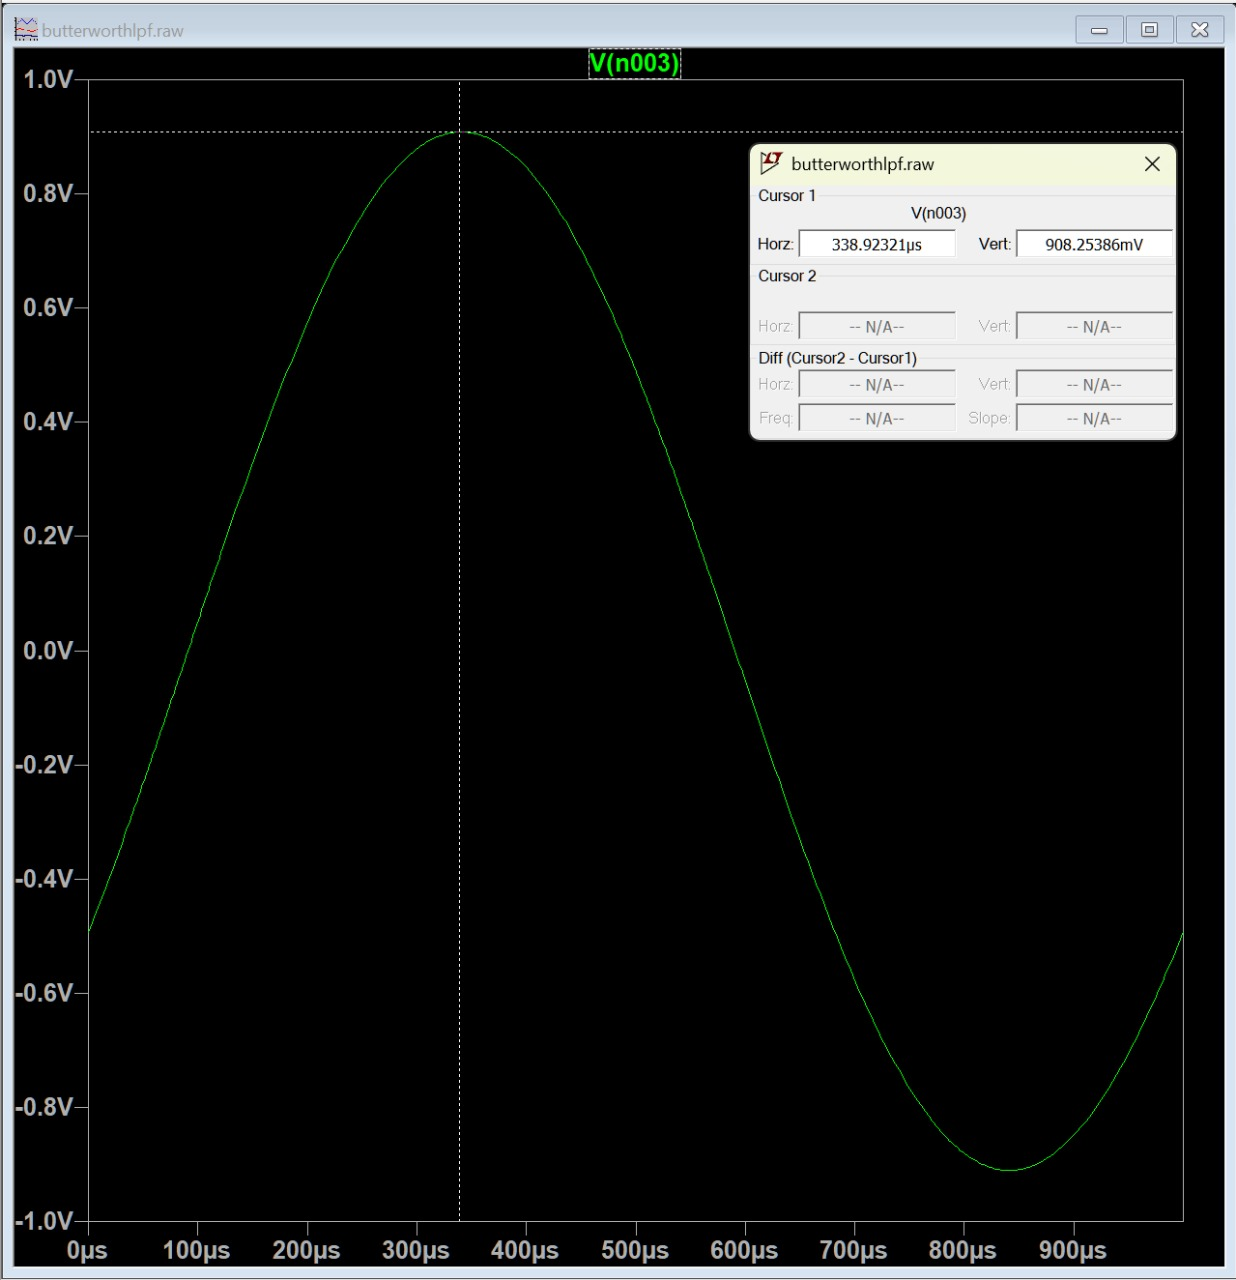
\includegraphics[width=1\linewidth]{WhatsApp Image 2025-05-03 at 23.00.41_3e6b0d50.jpg}
    \caption{for 1kHz, input amplitude is 1V, output amplitude is 908mV}
    \label{fig:enter-label}
\end{figure}
\begin{figure}[H]
    \centering
    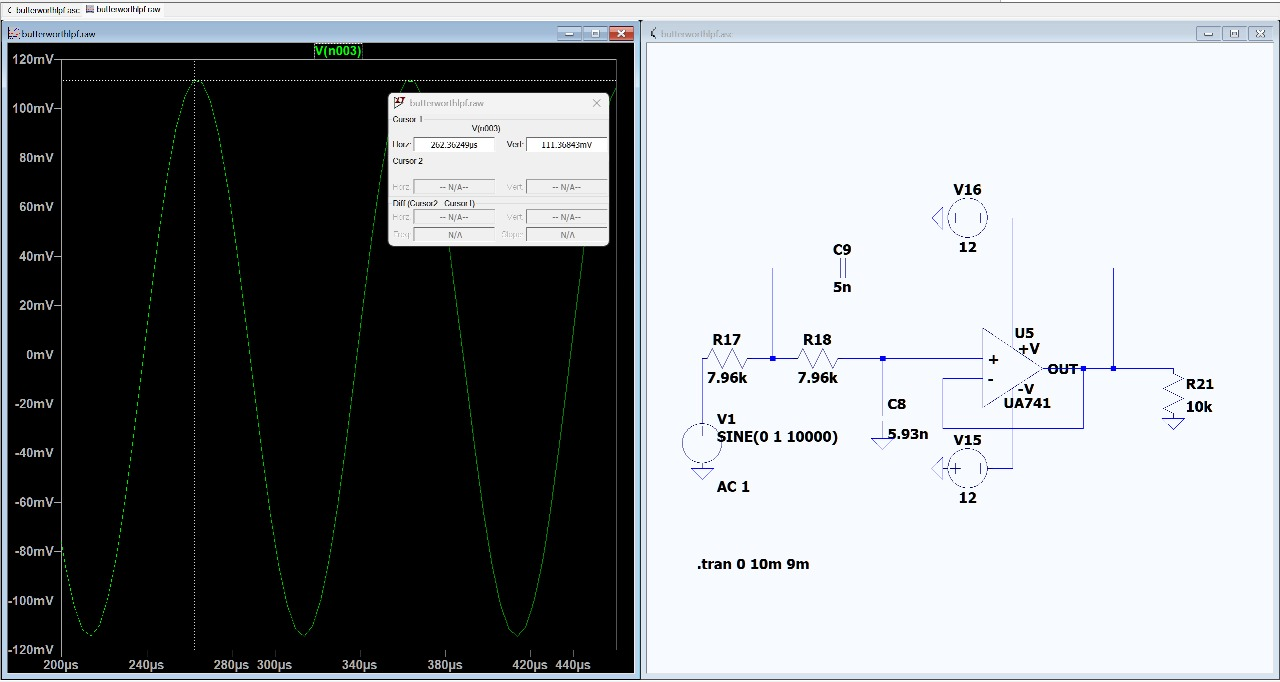
\includegraphics[width=1\linewidth]{WhatsApp Image 2025-05-03 at 23.01.42_8e5ea48b.jpg}
    \caption{10kHz, for input at 1V again, output is 111mV}
    \label{fig:enter-label}
\end{figure}
\begin{figure}[H]
    \centering
    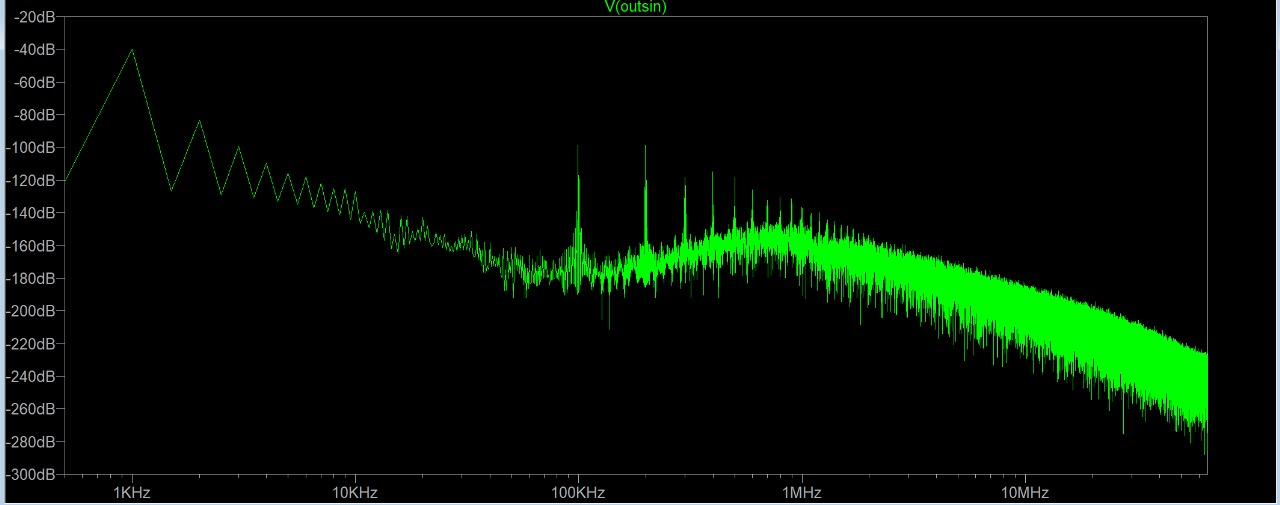
\includegraphics[width=1\linewidth]{cc.jpg}
    \caption{lpf mixed with mixer, 100k - 99k (1kHz), fft peaks at 1k properly}
    \label{fig:enter-label}
\end{figure}
\begin{figure}[H]
    \centering
    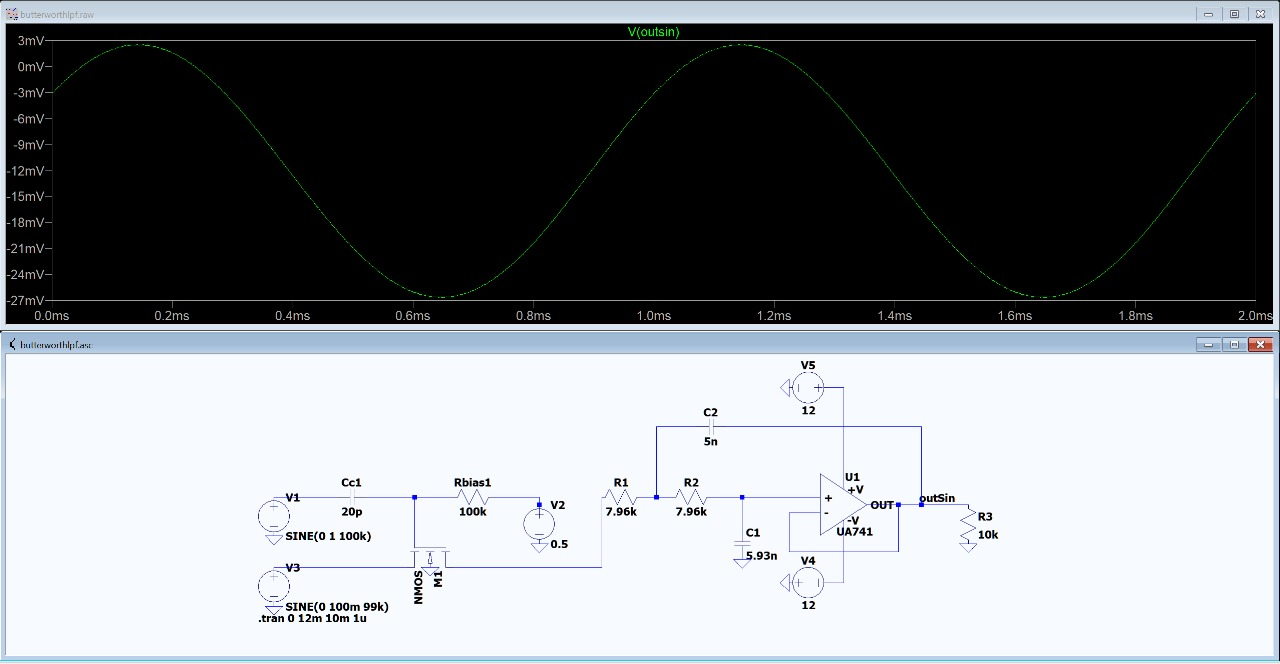
\includegraphics[width=1\linewidth]{dd.jpg}
    \caption{}
    \label{fig:enter-label}
\end{figure}

\section{Final Workflow}
All in All, We have 3 components fused together,
We take in an input signal and output the inphase and quadrature phase of the very same signal that we send as the output. To do so, the input signal is sent to two switches/mixer that multiply them to two sinusoidal waves differing with a 90\textdegree  phase difference by toggling repeatedly between saturation and triode region. Here specifically in the deep triode region where the drain current is directly proportional to the Drain-Source voltage (Deep Triode) region. The sinusoidal waves are generated by the Quadrature oscillator that uses a Wien bridge oscillation setup that generates the first sine wave and then a corresponding integrator circuit that generates a 90\textdegree phase shift and produces a -cosine wave. Now after being multiplied, both signals are passed through low pass filters that only selectively allows the desired frequencies and removes the higher-order frequency terms. This provides us with a clean result.
\begin{figure}[H]
    \centering
    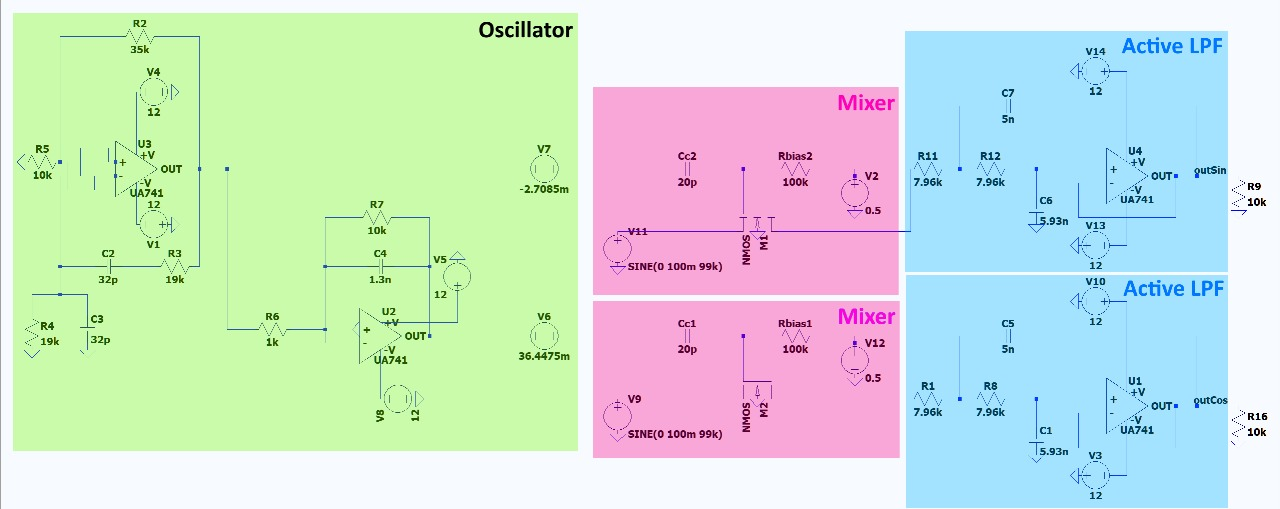
\includegraphics[width=1\linewidth]{aa.jpg}
    \caption{Classification of the final circuit}
    \label{fig:enter-label}
\end{figure}
\begin{figure}[H]
    \centering
    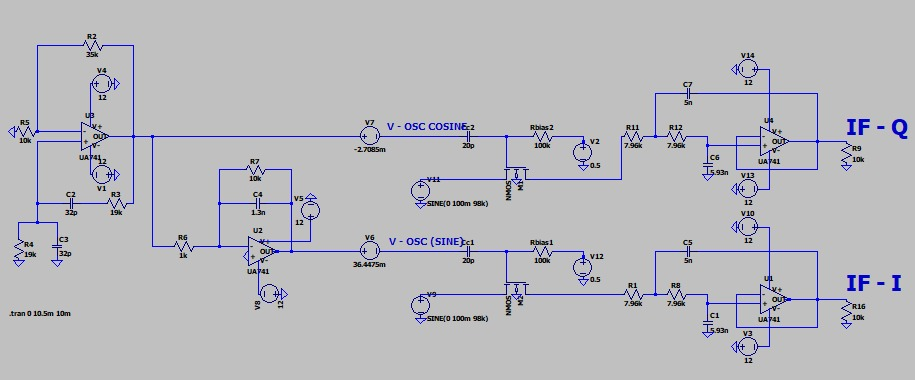
\includegraphics[width=1\linewidth]{ff.jpg}
    \caption{Final Circuit Diagram}
    \label{fig:enter-label}
\end{figure}
\begin{figure}[H]
    \centering
    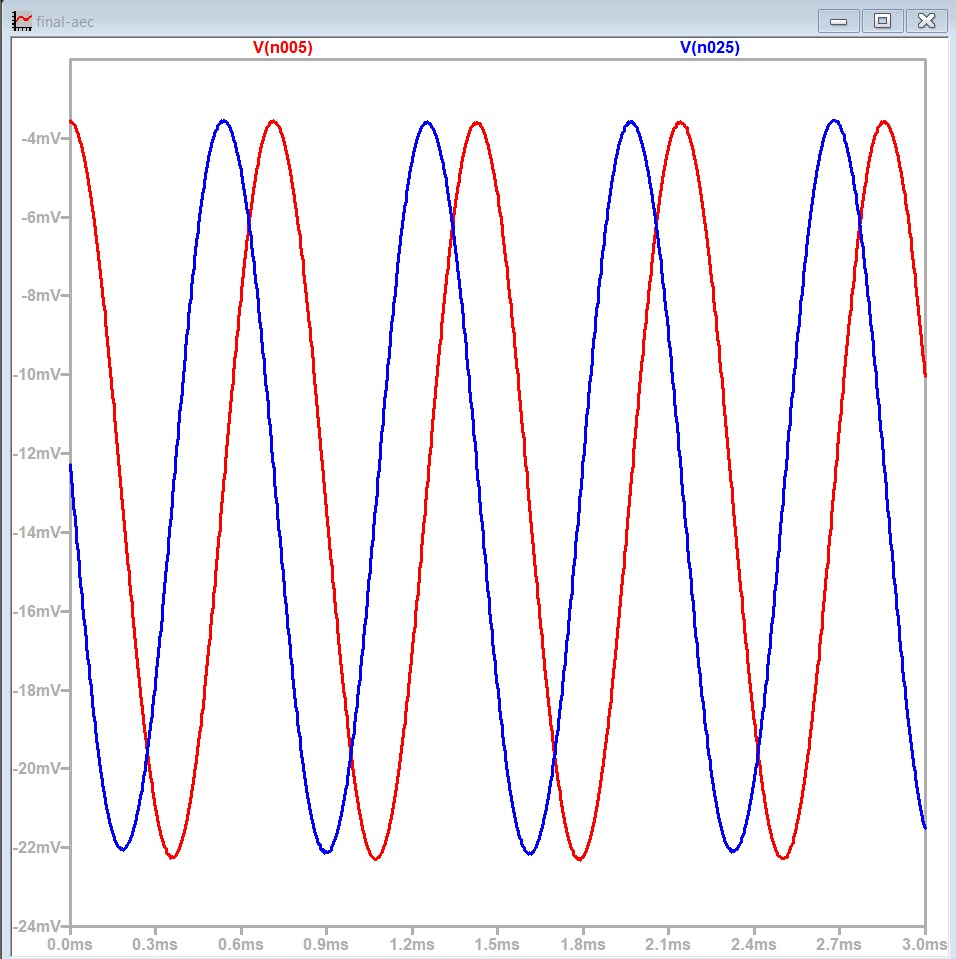
\includegraphics[width=0.8\linewidth]{WhatsApp Image 2025-05-03 at 21.22.53_a21fd795.jpg}
    \caption{Final Output form}
    \label{fig:enter-label}
\end{figure}
\begin{figure}[H]
    \centering
    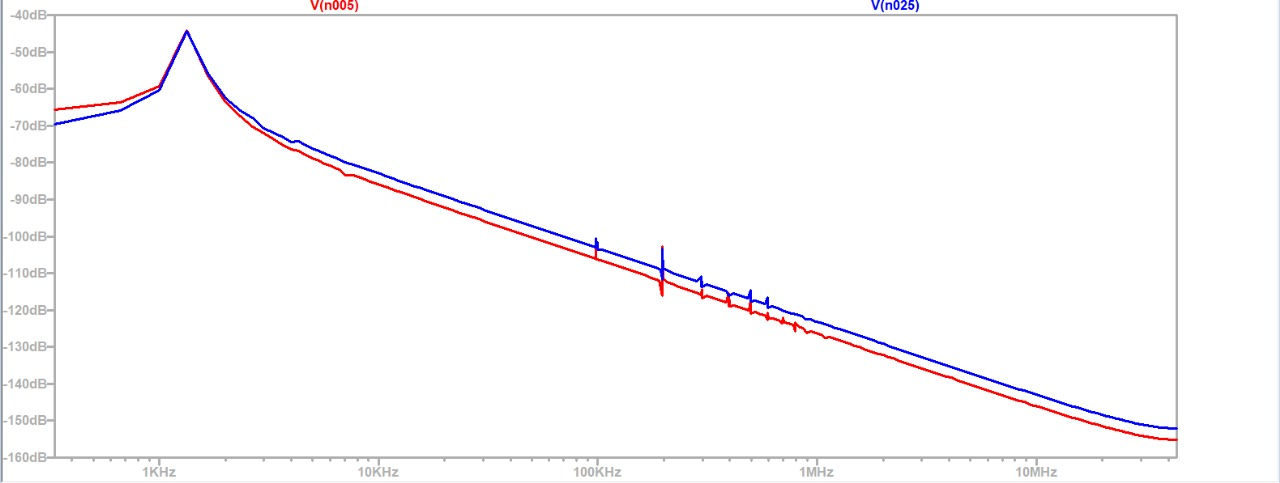
\includegraphics[width=0.8\linewidth]{WhatsApp Image 2025-05-03 at 22.10.09_d05123f5.jpg}
    \caption{FFT of the generated waveform}
    \label{fig:enter-label}
\end{figure}
\section{Acknowledgments}

The Authors of this paper would like to thank International 
Institute of Information Technology, Hyderabad for the 
sponsored access to several scientific websites like IEEE. 
Thanks are given to Prof. Zia Abbas for providing 
support and this platform to study and present ideas on this 
topic. The authors also give thanks to the teaching assistants of the Analog Electronic Circuits course of the Institute for their help and useful comments on the paper. 
\section{References}

[1] Design of Analog CMOS integrated Circuits by Behzad 
Razavi Chapter 2 and Chapter 4.  
[2] Rahsoft.com - understanding quadrature down conversion.  
[3] Babak Bastani, Edwin E Bautisa, Geetha Nagaraj and Joe 
Heck, “A Quadrature Down Converter For Direct Conversion 
Receivers with High 2nd and 3rd Order Intercept” IEEE.  
[4] Electricaltechnology.org – passive low pass filters.  
[5] Microelectronic Circuits by Adel S. Sedra, Kenneth C. 
Smith, Chapter 2 and Chapter 14.  
[6] Ron Mancini, “Design of op amp Sine Wave Oscillator”. 
Ralph Holzel, “A Simple Wde-Band Sine Wave Quadrature 
Oscillator” IEEE Transactions on Instrumentation and 
Measurement, vol. 42, pp.3, June 1993.
\end{document}